\documentclass[12pt, a4paper,onecolumn]{article}
% Use the option doublespacing or reviewcopy to obtain double line spacing
%\documentclass[doublespacing]{elsart}
% The amssymb package provides various useful mathematical symbols
\usepackage{amssymb}
\usepackage{amsmath}
\usepackage{epsfig}
\usepackage{caption}
\captionsetup{font=footnotesize}
\usepackage{epstopdf}
\usepackage{tabularx}
\usepackage{graphicx}
\usepackage{wrapfig}
\usepackage[numbers]{natbib}
\usepackage{courier}
\usepackage{hyperref}
\usepackage{tikz}
\usetikzlibrary{arrows.meta}

\usepackage{float}

\usepackage{listings}
\usepackage{color}

\definecolor{dkgreen}{rgb}{0,0.6,0}
\definecolor{gray}{rgb}{0.5,0.5,0.5}
\definecolor{mauve}{rgb}{0.58,0,0.82}

\lstset{frame=tb,
	language=C++,
	aboveskip=3mm,
	belowskip=3mm,
	showstringspaces=false,
	columns=flexible,
	basicstyle={\small\ttfamily},
	numbers=none,
	numberstyle=\tiny\color{gray},
	keywordstyle=\color{blue},
	commentstyle=\color{dkgreen},
	stringstyle=\color{mauve},
	breaklines=true,
	breakatwhitespace=true,
	tabsize=3
}

\newcommand{\Rmp}{\left<\mathbf{R}_p\right>}
\newcommand{\Rmpsq}{\left<\mathbf{R}_p^2\right>}
\newcommand{\tr}{\mathop{\mathrm{tr}}}
\def\vs{\vspace{0.1cm}\noindent}
\newcommand{\br}{\mathbf{r}}

\begin{document}
\begin{titlepage}
	\centering
	\vfill
	{\bfseries\Huge
		SPHinXsys User's Guide \\
		\vskip2cm
	}
	{\bfseries\Large
	Version $\boldsymbol{\alpha}$\\
	}
	{
		\bfseries\normalsize
		0.0.0\\
		\vskip1cm
		\today\\
	}    
	\vfill
	
\includegraphics[width=4cm]{figs/logo.eps} % also works with logo.pdf
	\vfill
	\vfill
\end{titlepage}

\clearpage

\vspace*{\fill}
%
\begin{wrapfigure}{l}{0.15\textwidth}
	\vspace*{-12pt}
	\scalebox{0.15}{
\includegraphics[width=\textwidth]{figs/logo.eps}}
	\vspace*{-12pt}
\end{wrapfigure}
%
\noindent Portions copyright \textcopyright\ 2019 Technical University of Munich, Xiangyu Hu, Luhui Han, Chi Zhang, Shuoguo Zhang, Massoud Rezavand.

\footnotesize{\noindent  Permission is hereby granted, free of charge, to any person obtaining a copy of this document (the "Document"), to deal in the Document without restriction, including without limitation the rights to use, copy, modify, merge, publish, distribute, sublicense, and/or sell copies of the Document, and to permit persons to whom the Document is furnished to do so, subject to the following conditions:

This copyright and permission notice shall be included in all copies or substantial portions of the Document.

THE DOCUMENT IS PROVIDED "AS IS", WITHOUT WARRANTY OF ANY KIND, EXPRESS OR IMPLIED, INCLUDING BUT NOT LIMITED TO THE WARRANTIES OF MERCHANTABILITY, FITNESS FOR A PARTICULAR PURPOSE AND NONINFRINGEMENT. IN NO EVENT SHALL THE AUTHORS, CONTRIBUTORS OR COPYRIGHT HOLDERS BE LIABLE FOR ANY CLAIM, DAMAGES OR OTHER LIABILITY, WHETHER IN AN ACTION OF CONTRACT, TORT OR OTHERWISE, ARISING FROM, OUT OF OR IN CONNECTION WITH THE DOCUMENT OR THE USE OR OTHER DEALINGS IN THE DOCUMENT.}
\clearpage

\newpage
\section*{Acknowledgement}
German Research Fundation (Deutsche Forschungsgemeinschaft) DFG HU1527/6-1, HU1527/10-1 and HU1527/12-1.

\newpage
\tableofcontents
%
\newpage
\section{Introduction}
\subsection{The code}
SPHinXsys (pronunciation: s'finksis) is an acronym from 
\underline{S}moothed \underline{P}article \underline{H}ydrodynamics 
for \underline{in}dustiral comple\underline{X} \underline{sys}tems.
It aims to model coupled industrial dynamic systems including fluid, 
solid, multi-body dynamics and beyond with SPH (smoothed particle hydrodynamics), 
a Lagrangian computational method using particle discretization.
The code presently includes fluid dynamics, solid dynamics, fluid-structure interactions (FSI), 
and their coupling to rigid-body dynamics (with Simbody library https://simtk.org).

%
\begin{wrapfigure}{r}{0.35\textwidth}
	\vspace*{-12pt}
	\scalebox{0.35}{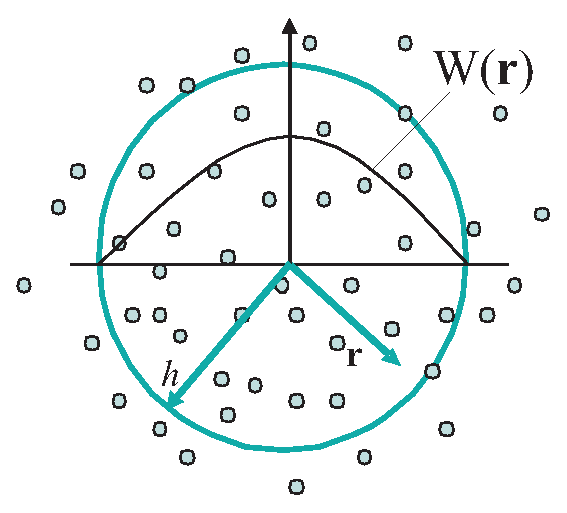
\includegraphics[width=\textwidth]{figs/sph.eps}}
	\caption{SPH particles and kernel function $W(\mathbf{r})$.}
	\label{figs:sph}
	\vspace*{-12pt}
\end{wrapfigure}
%
\subsection{Unified modeling for fluid and solid dynamics}
SPH is a fully Lagrangian particle method,  
in which the continuum media is discretized into Lagrangian particles
and the mechanics is approximated as the interaction between them
with the help of a kernel, usually a Gaussian-like function, as shown in Fig. \ref{figs:sph}. 
SPH is a mesh free method, which does not require a mesh to define 
the neighboring interaction configuration of particles, 
but construct or update it according to the distance between particles.
A remarkable feature of this method is that its computational algorithm 
involves a large number of common abstractions, e.g. particles,  
which link to many physical systems inherently. 
Due to such unique feature,
SPH have been used in SPHinxSys for unified continuum-mechanics 
modeling of both fluid and solid mechanics.

Generally, for continuum mechanics, 
we consider three types of media according their level of deformation.
\begin{itemize}
	\item The first type is rigid solid characterized by uniform translate and angular velocities. 
	\item The second type  is elastic solid characterized by regular velocity field and deformation-induced stress.
	\item The third type is fluid characterized by velocity-gradient-induced stress.
\end{itemize}
In SPHinxSys, all media are modeled as SPH bodies. 
Each body is composed of a group of SPH particles.
See Figure \ref{figs:fsi} for a typical example in a simulation.  
%
\begin{figure}[tb!]
	\centering
	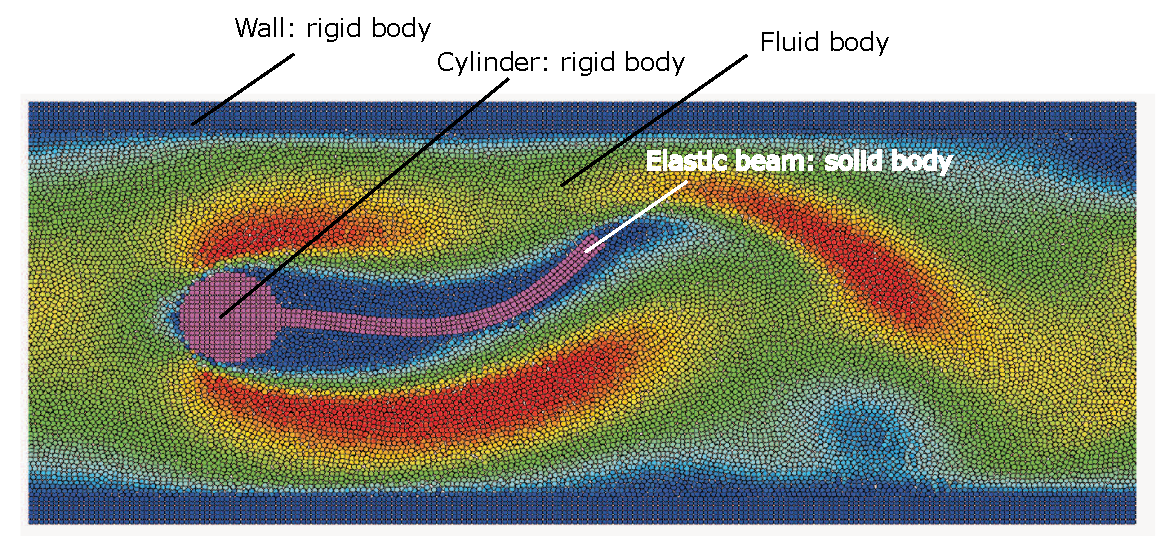
\includegraphics[width=\textwidth]{figs/fsi.eps}
	\caption{A typical FSI problem involving a rigid solid (wall) body, 
		a composite solid (insert) body and a fluid body. The wall body has two (upper and lower) components. 
		The insert body is composed of a rigid (cylinder) and an elastic (beam) components.}
	\label{figs:fsi}
\end{figure}
%
Note that a SPH solid body may be composed of than one components.
As shown in Fig. \ref{figs:fsi}, 
while the wall body has two rigid solid components,
the insert is composed of a rigid and an elastic solid components.

The SPH algorithms are used to discretize the continuum mechanics equations, 
and compute the dynamics of particles, i.e. their trajectory, velocity and acceleration. 
The algorithms for the discretization of the fluid dynamics equations are based on a weakly compressible fluid formulation, which is suitable for the problems with incompressible flows, and compressible flows with low Mach number (less than 0.3). The solid dynamics equations are discretized by a total Lagrangian formulation, which is suitable to study the problems involving linear and non-linear elastic materials. The FSI coupling algorithm is implemented in a kinematic-force fashion, in which the solid structure surface describes the material-interface and, at the same time, experiences the surface forces imposed by the fluid pressure and friction. 
SPHinxSys couples the rigid bodies with elastic solid and fluid in a kinematic-force fashion too,
in which, while experiencing forces from elastic solid and/or fluid, 
the rigid bodies and their interactions (handled by Simbody library) 
determines the position and velocity their own particles. 
%
\subsection{Multi-resolution modeling}
SPHinXsys carries out multi-resolution modeling 
by allowing different particle resolution for fluid and solid bodies. 
Subsequently, the fluid and solid dynamics equations are integrated with different time steps.
Note that SPHinXsys implements advanced algorithms 
such that the simulation is still simple, accurate, numerically stable and,
 more importantly, conserves momentum conservation globally and locally.
%
\subsection{Using this guide}
This user's guide is intended as a starting place for new SPHinXsys users. 
An overview of the theory and architecture of SPHinXsys is given in chapter \ref{theory}. 
Detailed installation instructions are provided in chapter \ref{install}, for Linux or Windows installation. Then a simple tutorial examples is given in chapter \ref{example}. Chapter \ref{complex-example} presents a more complex example, 
which exercises the FSI feature of SPHinXsys for performing studies on industrial problems.
%
\newpage
\section{SPHinXsys theory and architecture overview}\label{theory}  
\subsection{Lagrangian continuum mechanics}
In continuum mechanics, 
the form of conservation equation depends on the reference configuration,
in which the spatial differential (such as gradient) operators are directly defined. 
Based on the reference configuration, the spatial differential operators 
in other configurations can be obtained by coordinate transformation.
SPHinXsys solves the continuum equations in Lagrangian formulations, 
in which the observer is following the material points of the continuum \cite{Han2018}. 
There are two distinct Lagrangian formulations: one is total Lagrangian formulation (TLF) 
in which the initial configuration is used as reference; 
the other is updated Lagrangian formulation (ULF) 
in which the current configuration is used as reference.   
Generally, while TLF is more suitable for modeling solid-like dynamics,
i.e. the integrity or topology of a continuum medium is preserved, 
ULF is more suitable for fluid-like dynamics 
which includes fracture, contact and self-contact, Newtonian and non-Newtonian fluid dynamics. 
%
\subsubsection{TLF for solid-like dynamics}  
In a solid-like domain $\Omega^{s}$, the trajectory of a material point 
$\mathbf{r} \equiv \mathbf{r}(\mathbf{R},t)$, 
where $\mathbf{R}$ is its position in the initial configuration, is defined by
%
\begin{equation}\label{trajectory}
\frac{d \mathbf{r}}{d t}  =  \mathbf{v},
\end{equation}
%
where $\mathbf{v}\equiv\mathbf{v}(\mathbf{r})$ is the local velocity.
The starting point of TLF is the deformation gradient tensor defined by 
%
\begin{equation}\label{deformation-tensor}
\mathbb{F}  =  \nabla^{o} \mathbf{r} = \nabla^{o} \mathbf{U}  + \mathbb{I}.
\end{equation}
%
Here, $\nabla^{o} \equiv \frac{\partial}{\partial \mathbf{R}}$ 
is the gradient operators defined in the initial configuration 
and $\mathbf{U} = \mathbf{r} - \mathbf{R}$ is the displacement function.
The Green-Lagrangian strain tensor is defined by 
%
\begin{equation}\label{Lagrangian-strain}
\mathbb{E}  = \frac{1}{2} \left(\mathbb{F}^{T}\mathbb{F} - \mathbb{I}\right) = \frac{1}{2} \left(\mathbb{C} - \mathbb{I}\right),
\end{equation}
%
where $\mathbb{C}$ is the right Cauchy deformation tensor.
The mass conservation equation is 
%
\begin{equation}\label{mass-conservation}
\rho  =  \det(\mathbb{F})^{-1}\rho_0,
\end{equation}
%
where $J = \det(\mathbb{F}) = \sqrt{\det(\mathbb{C})}$ is the Jacobian determinant. 
The momentum conservation equation is 
%
\begin{equation}\label{momentum-conservation}
\frac{d \mathbf{v}}{d t}  = \frac{1}{\rho_0}\nabla^{o} \cdot \mathbb{P} + \mathbf{g},
\end{equation}
%
where $\mathbb{P}$ is the 1st Piola- Kirchhoff stress tensor 
which relates forces in the current configuration with areas in the initial configuration.
Note that Eq. (\ref{mass-conservation}) is redundant and not required for solving Eq. (\ref{momentum-conservation}). 
For linear elastic or Kirchhoff materials, $\mathbb{P}$ can be obtained by 
%
\begin{equation}\label{linear-elasticity}
\mathbb{P} = \mathbb{F} \mathbb{S}, \quad \mathbb{S}  = \boldsymbol{\mathsf{C}}:\mathbb{E} ,
\end{equation}
%
where $\mathbb{S}$ is the 2nd Piola- Kirchhoff stress,
which relates with Cauchy stress by
%
\begin{equation}\label{2nd-PK-Cauchy}
\mathbb{S} = \mathbb{F}^{-1} J \mathbb{\sigma} \mathbb{F}^{-T},
\end{equation}
% 
and $\mathbb{S}  = \boldsymbol{\mathsf{C}}:\mathbb{E}$ is called constitute relation 
in which $\boldsymbol{\mathsf{C}}$ is the a constant 4th-rank elasticity tensor. 
When the material is isotropic, the  constitute relation reduces to
%
\begin{eqnarray}\label{isotropic-linear-elasticity}
\mathbb{S} & = & K (\tr \mathbb{E}) \mathbb{I} + 2 G (\mathbb{E} - \frac{1}{3}(\tr \mathbb{E}) \mathbb{I}) \nonumber\\
& = & \lambda (\tr \mathbb{E}) \mathbb{I} + 2 \mu \mathbb{E}
\end{eqnarray}
%
where $K = \lambda + 2\mu/3$ is the bulk modulus and $G = \mu$ is the shear modulus. 

A more involved constitutive model is the Neo-Hookean model,
which is defined by the strain energy with the form
%
\begin{eqnarray}\label{Neo-Hookean-energy}
W & = & \frac{\mu}{2}(I_1 - 3 - 2 \ln J) + \frac{\lambda}{2}(\ln J)^{2} \nonumber\\
& = & \mu \tr \mathbb{E} - \mu \ln J + \frac{\lambda}{2}(\ln J)^{2}
\end{eqnarray}
%
where $I_1 = \tr \mathbb{C}$ is the first principle invariant.
To take into account the finite extensibility, 
the strain energy can be modified to
%
\begin{equation}\label{Neo-Hookean-energy-finite-extensibility}
W = -\frac{\mu}{2}J^{1}_{m}\ln \left(1 - \frac{I_1 - 3}{J^{1}_{m}}\right)  - \mu\ln J + \frac{\lambda}{2}(\ln J)^{2}
\end{equation}
%
where $J^{1}_{m}$ is the parameter to define the maximum extensibility.
The stress-strain relation defined by strain energy is
%
\begin{eqnarray}\label{stress-strain-energy}
\mathbb{S}  = \frac{\partial W}{\partial \mathbb{E}} = 2\frac{\partial W}{\partial \mathbb{C}}
& =  &2\frac{\partial W}{\partial I_1}\frac{\partial I_1}{\partial \mathbb{C}} 
+ 2\frac{\partial W}{\partial J}\frac{\partial J}{\partial \mathbb{C}} \nonumber\\
& = & 2\frac{\partial W}{\partial I_1} \mathbb{I} + \frac{\partial W}{\partial J} J \mathbb{C}^{-1}   \\
& = & \mu \left(1 - \frac{2(\tr \mathbb{E})}{J^{1}_{m}}\right)^{-1} \mathbb{I} + (\lambda \ln J - \mu) \mathbb{C}^{-1}. \nonumber
\end{eqnarray}
%
A further involved constitutive model is the muscle model, 
in which the layered organization is characterized by a right-handed orthonormal set of
basis vectors and an associated orthogonal curvilinear system of coordinates. 
The local fixed set of (unit) basis vectors consists of the fibre axis  $\mathbf{f}_0$, which coincides
with the muscle fibre orientation, the sheet axis $\mathbf{s}_0$, defined to be in the plane
of the layer perpendicular to the fibre direction (sometimes referred to as the
cross-fibre direction), and the sheet-normal axis $\mathbf{n}_0$, defined to be orthogonal to the other two.
Due to the directional preferences, besides the principle invariants,
%
\begin{equation}\label{principle-invariants}
I_1 = \tr \mathbb{C}, \quad I_2 = \frac{1}{2}\left[I^2_1 - \tr(\mathbb{C}^2)\right], \quad I_3 = \det(\mathbb{C}) = J^2,
\end{equation}
%
there are other 3 independent invariants
%
\begin{equation}\label{extra-principle-invariants}
I_{ff}  =   \mathbb{C} : \mathbf{f}_0 \otimes\mathbf{f}_0,
\quad I_{ss}  =   \mathbb{C} : \mathbf{s}_0 \otimes\mathbf{s}_0,
\quad I_{fs}  =   \mathbb{C} : \mathbf{f}_0 \otimes\mathbf{s}_0.
\end{equation}
%
A typical strain energy for muscle has the form
%
\begin{eqnarray}\label{muscle-energy}
W  & = &  \frac{a}{2b}\exp\left[b (I_1 - 3 - 2\ln J)\right]  + \frac{\lambda}{2}(\ln J)^{2} \nonumber\\
&+& \sum_{i=f,s} \left\{\frac{a_i}{2b_i}\exp\left[b_i (I_{ii} - 1)^2\right] - 1 \right\} \\
&+ &\frac{a_{fs}}{2b_{fs}}\left[\exp(b_{fs} I^2_{fs}) - 1 \right], \nonumber
\end{eqnarray}
%
and the stress-strain relation is
%
\begin{eqnarray}\label{stress-strain-energy}
\mathbb{S} & = &  a\exp\left[b (I_1 - 3 - 2\ln J)\right] \mathbb{I} \nonumber \\
& + & \left\{ \lambda\ln J - a\exp\left[b (I_1 - 3 - 2\ln J)\right]\right\}\mathbb{C}^{-1}\nonumber\\
&+& 2 a_f(I_{ff} - 1)\exp\left[b_f (I_{ff} - 1)^2\right] \mathbf{f}_0 \otimes\mathbf{f}_0\\
&+& 2 a_s(I_{ss} - 1)\exp\left[b_s (I_{ss} - 1)^2\right] \mathbf{s}_0 \otimes\mathbf{s}_0\nonumber\\
&+ &a_{fs}I_{fs}\left[\exp(b_{fs} I^2_{fs})\right] 
(\mathbf{f}_0 \otimes\mathbf{s}_0 + \mathbf{s}_0 \otimes\mathbf{f}_0).\nonumber
\end{eqnarray}
% 
where $a$, $b$, $a_{ff}$,$b_{ff}$, $a_{ss}$, $b_{ss}$, $a_{fs}$ and $b_{fs}$ are 
the parameters of the orthotropic Holzapfel model \cite{holzapfel2009constitutive}.
Note that $\mu = ab$ is the shear modulus of 
the background isotropic Neo-Hookean constitutive relation.

During dynamical deformation, the elastic solid experience damping.
A typical model for such phenomenon is the Kelvin–Voigt model, 
which consists of elastic and damping stresses.
The latter is proportional to the strain rate.
%
\begin{equation}\label{solid-damping}
\mathbb{S}^{D} = \eta \dot{\epsilon} = \frac{\eta}{2} \left(\dot{\mathbb{F}}^{T}\mathbb{F} + \mathbb{F}^{T}\dot{\mathbb{F}} \right)
\end{equation}
%
where $\eta$ is the damping coefficient with the same dimension of fluid dynamical viscosity.
%
\subsubsection{ULF for fluid-like dynamics}  
The starting point of ULF is the velocity gradient tensor and strain rate tensor defined, respectively, by 
%
\begin{equation}\label{strain-rate-tensor}
\mathbb{L} = (\nabla \mathbf{v})^{T}, \quad \mathbb{D}  = \frac{1}{2} (\mathbb{L}+ \mathbb{L}^{T}).
\end{equation}
%
Here, $\nabla \equiv \frac{\partial}{\partial \mathbf{r}}$ 
is the gradient operators defined in the current configuration.
The mass conservation equation is
%
\begin{equation}\label{mass-conservation-ULF}
\frac{d \rho}{d t}  = -\rho \nabla \cdot\mathbf{v}.
\end{equation}
%
The momentum conservation equation is 
%
\begin{equation}\label{momentum-conservation-ULF}
\frac{d \mathbf{v}}{d t}  = -\frac{1}{\rho}\nabla p + \frac{1}{\rho}\nabla \cdot \boldsymbol{\tau} + \mathbf{g},
\end{equation}
%
where $p = c^2_0(\rho - \rho_0)$, $c_0$ is sound speed, 
is pressure and $\boldsymbol{\tau}$ the shear stress. 
Note that, for weakly compressible fluids,  
$c_0$ is chosen much larger than the characteristic speed of the dynamics
and one has $\boldsymbol{\tau} = 2\mu \mathbb{D}$ 
and $\nabla \cdot \boldsymbol{\tau} = \mu \nabla^{2} \mathbf{v}$.
For non-Newtonian fluid, for example Oldroyd-B fluid,
the shear stress is determined by 
%
\begin{equation}\label{non-Newtonian-shear-stress}
\boldsymbol{\tau} = 2 \mu_s\mathbb{D} + \boldsymbol{\tau}_p, \quad \boldsymbol{\tau}_p + \lambda \overset{\scriptscriptstyle{\nabla}}{\boldsymbol{\tau}_p} = 2\mu_p \mathbb{D},
\end{equation}
%
where $\mu_s$ is viscosity of the solvent, $\mu_p$ is polymer contribution to viscosity at zero shear rate,
$\lambda$ is the relaxation time and 
$ \overset{\scriptscriptstyle{\nabla}}{\boldsymbol{\tau}_p} = d \boldsymbol{\tau}_p /dt 
- (\mathbb{L}^{T}\cdot \boldsymbol{\tau}_p +  \boldsymbol{\tau}_p \cdot \mathbb{L})$ is  
the upper convected time derivative of the polymer shear stress tensor.
Since non-Newtonian fluid is also weakly compressible, Eq. (\ref{non-Newtonian-shear-stress}) can be further approximated as
%
\begin{equation}\label{non-Newtonian-shear-stress-simplified}
\nabla \cdot \boldsymbol{\tau} = \mu_s\nabla^{2} \mathbf{v} + \nabla \cdot \boldsymbol{\tau}_p, 
\quad \nabla \cdot \boldsymbol{\tau}_p + \lambda \overset{\scriptscriptstyle{\nabla}}{(\nabla \cdot \boldsymbol{\tau}_p)} = \mu_p \nabla^{2} \mathbf{v}.
\end{equation}
%
\subsection{Basic SPH discretizations}
In SPH modeling, a variable field $\psi(\mathbf{r})$ in a continuum medium 
is discretized with a particle system   
%
\begin{equation}
\psi_i  = \int \psi(\mathbf{r}) W(\mathbf{r} - \mathbf{r}_i, h)d\mathbf{r}. 
\label{particle-average}
\end{equation}
%
Here, $i$ is the particle index, $\psi_i$ is the discretized particle-average variable,  
$\mathbf{r}_{i}$ is the position of the particle.
The compact-support kernel function $W(\mathbf{r}_{i} - \mathbf{r}, h)$, 
where $h$ is the smoothing length related with cut-off radius by $r_c = \alpha h$, 
$a>1$ is a small integer number, 
is radially symmetric respect to $\mathbf{r}_{i}$,
and has the properties $\int W(\mathbf{r}_{i} - \mathbf{r}, h)
d\mathbf{r} =1 $, $\int\nabla W(\mathbf{r}_{i} - \mathbf{r})d\mathbf{r} = \mathbf{0}$ 
and $\lim_{h\rightarrow 0}W(\mathbf{r}_{i} - \mathbf{r}, h) = \delta(\mathbf{r}_{i} - \mathbf{r})$,
the Dirac delta function.
Since we assume that the mass of each particle $m_i$ is known and invariant (indicating mass conservation),
one has the particle volume $V_i = m_i/\rho_i$, where $\rho_i$ is the particle-average density.

It is also assumed, in SPH modeling, a reconstruction method to approximate 
a variable from the particle-average values by
%
\begin{equation}
\psi(\mathbf{r}) \approx \sum_{j\in s}  V_j W(\mathbf{r} - \mathbf{r}_{j}, h)\psi_j = \sum_{j\in s}  \frac{m_j}{\rho_j} W(\mathbf{r} - \mathbf{r}_{j}, h)\psi_j, 
\label{particle-reconstuction}
\end{equation}
%
where the summation is for all the partilces $j$ in the neighborhood region $s$ within a cut-off radius, 
and leads to an approximation of the particle-average density 
%
\begin{equation}
\rho_i \approx \sum_{j\in s}  m_j W_{ij}, 
\label{particle-density-reconstuction}
\end{equation}
%
which is an alternative way to update fluid density other than the evolution equation of Eq. (\ref{mass-conservation-ULF}).
Due to different level of deformation, 
evaluating density within a body should only taking into account 
particle motion within its own and the stiffer neighboring bodies.
For example, the density of a solid particle can only taking into 
account the effects from its neighboring particles within its own and rigid bodies. 

The dynamics of other particle-average variables
is based on a general form of interaction between the particle $i$ and its neighboring particles,
i.e. the approximation of the spatial derivative operators on the right-hand-sides of the their evolution equations.
The original SPH approximation of the derivative of a variable field $\psi(\br)$ at a particle $i$  is obtained by 
the following,
%
\begin{equation}
\label{eq:gradsph}
\nabla \psi_i \approx \int_{V} \nabla \psi (\br) W(\br_i - \br, h) dV  
=  - \int_{V} \psi (\br) \nabla W(\br_i - \br, h) dV
\approx  - \sum_{j\in s}  V_j \nabla W_{ij}\psi_j . 
\end{equation}
%
Here, $\nabla \psi_i \equiv  \nabla \psi(\br_i)$, $\psi_j \equiv \psi (\br_j)$ 
and $\nabla W_{ij} \equiv \nabla W(\br_i - \br_j, h)\equiv \nabla W(r_{ij} \mathbf{e}_{ij}, h)$, 
where $r_{ij}$ and $\mathbf{e}_{ij}$ are the distance 
and unit vector of the particle pair $(i,j)$, respectively.
Note that, when a boundary intersects the kernel support, 
the application of Eqs. (\ref{eq:gradsph})
requires a proper boundary condition to define the field outside of the boundary.

In SPH modeling \cite{hu2015towards}, the original approximation of Eq. (\ref{eq:gradsph}) is modified into a strong form
%
\begin{equation}
\label{eq:gradsph-strong}
\nabla \psi_i = \psi_{i}\nabla 1 + \nabla \psi_i \approx   \sum_{j\in s} V_j \nabla W_{ij} \psi_{ij}, 
\end{equation}
%
where $\psi_{ij} = \psi_{i} - \psi_{j}$ is the inter-particle-difference value. 
The strong-form approximation of the derivative is used to determine the local structure of a field.
With a slight different modification, 
the original approximation of Eq. (\ref{eq:gradsph}) is rewritten into an weak form
%
\begin{equation}
\label{eq:gradsph-weak}
\nabla \psi_i = \nabla \psi_i - \psi_{i}\nabla 1 \approx   -2\sum_{j\in s}  V_j\nabla W_{ij} \overline{\psi}_{ij}, 
\end{equation}
%
where $\overline{\psi}_{ij} = \left(\psi_{i} + \psi_{j}\right)/2$ is the inter-particle-average value. 
The weak-form approximation of derivative is used to computed the surface integrations respected to a variable 
for solving its conservation law.
Due to the anti-symmetric property of the derivative of the kernel function, 
i.e. $\nabla W_{ij} = - \nabla W_{ji}$, it implies momentum conservation of the particle system.
%
\subsubsection{Discretization of TLF conservation equations}
The discretization is based on the approximation of 
the displacement gradient and divergence of the 1st Piola- Kirchhoff stress tensor, 
respectively, in Eqs. (\ref{deformation-tensor})  and (\ref{momentum-conservation}). 
A strong formulation is used to approximate the displacement gradient as 
%
\begin{equation}\label{sph-displacement-gradient}
\left(\nabla^{o} \mathbf{U}\right)_i \approx  \sum_{j\in s^{o}}  \mathbf{U}_{ij} \otimes  \nabla W^{o}_{ij} V^{o}_j,
\end{equation}
%
where $W^{o}_{ij}$ and $V^{o}_j$ are evaluated in the initial configuration with the neighborhood $s^{o}$.
Note that in order to reproducing the rotation of rigid body, 
Eq. (\ref{sph-displacement-gradient}) is further corrected by
%
\begin{equation}\label{sph-displacement-gradient-corrected}
\left(\nabla^{o} \mathbf{U}\right)_i \approx   \left(\sum_{j\in s^{o}} \mathbf{U}_{ij} \otimes  \nabla W^{o}_{ij}V^{o}_j\right)\mathbb{B}_i.
\end{equation}
%
The expression of the correction term is 
%
\begin{equation}\label{sph-gradient-correction}
\mathbb{B}_i =  \left(\sum_{j\in s^{o}} \mathbf{R}_{ij} \otimes V\nabla W^{o}_{ij}V^{o}_j \right)^{-1}.
\end{equation}
%
A weak form is used for approximating the divergence of the 1st Piola- Kirchhoff stress tensor as
\begin{equation}
\label{eq:surface-integral-TFL}
\nabla^{o} \cdot \mathbb{P}_i \approx 
-2 \sum_{j\in s^{o}}  \overline{\mathbb{P}}_{ij} \cdot \nabla W^{o}_{ij} V^{o}_j.
\end{equation}
%
\subsubsection{Discretization of UFL conservation equations}
%
The approximation of
the strain rate tensor in Eq. (\ref{strain-rate-tensor})
can be written is a strong form as
%
\begin{equation}\label{sph-strain-rate-tensor}
\mathbb{L}_i \approx   \sum_{j\in s} \bold{v}_{ij} \otimes \nabla W_{ij}  V_j,
\end{equation}
%
where the kernel function $ W_{ij}$ and particle volume $V_j$ are evaluated at the current configuration.
We introduce a further correction to increase the reproducing property by
 %
 \begin{equation}\label{sph-strain-rate-tensor-corrected}
 \mathbb{L}_i \approx  d \left(\sum_{j\in s} \bold{R}_{ij} \cdot \nabla W_{ij}  V_j\right)^{-1} \sum_{j\in s} \bold{v}_{ij} \otimes \nabla W_{ij}  V_j,
 \end{equation}
 %
where $d=3$ is the dimensions.
Note that this discretization is also used to approximate the velocity divergence from Eq. (\ref{mass-conservation-ULF}).
A weak form is used to approximate the pressure gradient form Eq. (\ref{momentum-conservation-ULF}) can be written as
%
\begin{equation}
\label{eq:surface-integral}
\nabla p_i \approx 
-2 \sum_{j\in s}  \overline{p}_{ij} \nabla W_{ij} V_j,
\end{equation}
%
and the Laplacian operator for the viscous force
%
\begin{equation}
\label{eq:gradsph-weak-Laplacian}
\nabla^2 \mathbf{v}_i \approx  
-2(d+2)\sum_{j\in s}\frac{\mathbf{v}_{ij}\cdot \mathbf{e}_{ij}}{r_{ij}} \nabla W_{ij}  V_j. 
\end{equation}
%
Note that this formulation reproduces constant and pure rotational flows.
%
\subsubsection{Modeling contact dynamics}
One issue for solid-like dynamics is the contact force, 
which prevents the over-crossing of solid bodies and introduces surface friction. 
A simple SPH model for this is based on ULF. 
We define a contact density for particles in a solid-like domains by 
%
\begin{equation}
\rho^{c}_i \approx  m_i\sum_{j\notin s^{o} \cap j\in s}  W_{ij}. 
\label{particle-density-conatct}
\end{equation}
%
where the summation is for those particles in solid-like domains and within the neighborhood of the current configuration 
but outside the neighborhood of the initial configuration, 
i.e. $r_{ij} < r_c$ and $r^{0}_{ij} > r_c$. 
As an analog to fluid-like dynamics, the contact dynamics is then defined as
%
\begin{equation}\label{momentum-conservation-contact}
\frac{d \mathbf{v}^{c}_{i}}{d t}  = -\frac{2}{\rho^{c}}\sum_{j\notin s^{o} \cap j\in s}  \overline{p^{c}}_{ij} \nabla W_{ij} V^{c}_j + \frac{2(d+2) \mu^{c}}{\rho^{c}}\sum_{j\notin s^{o} \cap j\in s}\frac{\mathbf{v}_{ij}\cdot \mathbf{e}_{ij}}{r_{ij}} \nabla W_{ij}  V^{c}_j, 
\end{equation}
%
where $V^{c}_i = m_i/\rho^{c}_i$ is contact volume, $p^{c}_{i}= c^2_0 \rho^{c}$ is contact pressure and $\mu^{c}$ is contact friction coefficient 
which can be related to contact pressure for more realistic friction models.
Note that this formulation also takes into account the self-contact dynamics.
%
\subsubsection{SPH discretization as coarse-graining model}
Assume that the continuum field is coarse-grained into a particle system 
with spatial filtering \cite{hu2012sph}, the variables on particles are obtained by
%
\begin{equation}
\psi_i  =  G_i * \psi  =  \int \psi(\mathbf{r}) W(\mathbf{r} - \mathbf{r}_i, h)d\mathbf{r}, 
\label{filtering}
\end{equation}
%
where $\mathbf{r}_{i}$ and $h$ are the center and width, respectively, of the filter.
Note that this filter can also take the role as the SPH kernel function with smoothing length $h$. 
Substitute $\psi(\mathbf{r})$ with the coordinate $\mathbf{r}$ into Eq. (\ref{filtering}),
that is
%
\begin{equation}\label{filtered-particle-position}
\mathbf{r}_i  =  G_i * \mathbf{r}  =  \int \mathbf{r} W(\mathbf{r} - \mathbf{r}_i, h)d\mathbf{r}, 
\end{equation}
%
one has the particle position $\mathbf{r}_i$ at the center of the filter.
The motion of particle is determined by its transport velocity, i.e.
%
\begin{equation}\label{particle-trajectory}
\frac{\widetilde{d} \mathbf{r}_i} {dt} =  \widetilde{\mathbf{v}}_i.
\end{equation}
%
Note that $\widetilde{\mathbf{v}}_i$ can be different from the filtered or momentum particle velocity $\mathbf{v}_i$,
which is obtained by substitute $\psi$ with velocity $\mathbf{v}$ into Eq. (\ref{filtering}), 
that is
%
\begin{equation}\label{momentum-particle-velocity}
\mathbf{v}_i  =  G_i * \mathbf{v}  =  \int \mathbf{v}(\mathbf{r}) W(\mathbf{r} - \mathbf{r}_i, h)d\mathbf{r}. 
\end{equation}
%
Similarly, the filtered derivatives on particles can be written as
%
\begin{eqnarray}
G_i * \nabla \psi & = & \int \nabla\psi W(\mathbf{r} - \mathbf{r}_i, h)d\mathbf{r} \nonumber \\
& = & - \int \psi \nabla W(\mathbf{r} - \mathbf{r}_i, h)d\mathbf{r}, \label{derivative} \\
G_i * \frac{d \psi}{dt} & = & \frac{\partial \psi_i}{\partial t}  + \int \nabla\psi\cdot \mathbf{v} W(\mathbf{r} - \mathbf{r}_i, h)d\mathbf{r} \nonumber \\
& = & \frac{\partial \psi_i}{\partial t} - \int \psi \mathbf{v}\cdot \nabla W(\mathbf{r} - \mathbf{r}_i, h)d\mathbf{r}, \label{full-derivative} 
\end{eqnarray}
%
Note that Eq. (\ref{full-derivative}) assumes the incompressibility, 
i.e. the velocity field is divergence free.
Since only the filtered values $\psi_i$ are known for the particle system, 
it is impossible to apply the exact filtering $G_i * \nabla \psi$ and $G_i * d\psi/d t$,
an approximated filtering is carried out after the flow field is first reconstructed 
%
\begin{equation}
\psi(\mathbf{r})  \approx  \frac{\sum_j\psi_j W(\mathbf{r} - \mathbf{r}_j)}{\sum_k W(\mathbf{r} - \mathbf{r}_k)}
= \frac{1}{\sigma}\sum_j\psi_j W(\mathbf{r} - \mathbf{r}_j),
\label{reconstruction} 
\end{equation}
where 
$\sigma = \sum_k W(\mathbf{r} - \mathbf{r}_k)$ 
is a measure of particle number density,
which is larger in a dense particle region than in a
dilute particle region \cite{KoshizukaNobeOka1998}.
From the identity $\sum_j W(\mathbf{r} - \mathbf{r}_j)/\sigma = 1$,
the total volume $V$ can be written as
%
\begin{equation}\label{volume}
V = \sum_j V_j = \sum_j \int\frac{1}{\sigma}W(\mathbf{r} - \mathbf{r}_j)d\mathbf{r} \approx \sum_j \frac{1}{\sigma_j}, 
\end{equation}
%
where $\sigma_j$ equals to the inverse of particle volume approximately, i.e. $\sigma_j = \sum_k W(\mathbf{r}_j - \mathbf{r}_k) = \sum_k W_{jk} \approx 1/V_j$. 
With Eq. (\ref{derivative}) and by using Eq. (\ref{reconstruction}) and the properties of the kernel function, 
the approximation of $G_i * \nabla \psi$ can be obtained by
%
\begin{eqnarray}
G_i *\nabla \psi  & \approx & - \sum_j \psi_{j}  \int\frac{1}{\sigma}\nabla W(\mathbf{r} - \mathbf{r}_i)W(\mathbf{r} - \mathbf{r}_j)d\mathbf{r} \approx - \sum_j  \psi_{j} \nabla W_{ij} V_j. \label{approx-derivative}
\end{eqnarray}
%
Note that Eq. (\ref{approx-derivative}) is a typical SPH discretization of the gradient operator.
Using particle transport velocity $\widetilde{\mathbf{v}}_{i}$, $G_i * d\psi/d t$ can be rewritten as
%
\begin{eqnarray}
G_i *\frac{d \psi}{dt} & \approx & \frac{\partial \psi_i}{\partial t}  - \sum_j  \psi_{j} \mathbf{v}_{j} \nabla W_{ij} V_j  \nonumber \\
& \approx & \frac{\partial \psi_i}{\partial t} + \widetilde{\mathbf{v}}_{i}\cdot \nabla \psi_i 
- \sum_j  \psi_{j} (\mathbf{v}_{j} - \widetilde{\mathbf{v}}_{j}) \nabla W_{ij} V_j, \nonumber \\
& \approx & \frac{\widetilde{d} \psi}{dt} - \sum_j  \psi_{j} (\mathbf{v}_{j} - \widetilde{\mathbf{v}}_{j}) \nabla W_{ij} V_j.
\label{approx-full-derivative}
\end{eqnarray}
%
Note that Eq. (\ref{approx-full-derivative}) assume the incompressible condition, 
i.e. $\nabla \cdot \widetilde{\mathbf{v}}_{i} = 0$ or the variation of particle density $\widetilde{d} \rho/dt = 0$.
Also note that the approximations in Eqs. (\ref{approx-derivative}) and (\ref{approx-full-derivative}) can be further modified into strong and weak forms.  
%
\subsubsection{Transport-velocity formulation}
Using Eq. (\ref{volume}), the particle density is given by
%
\begin{equation}\label{density_summation}
\rho_{i} = m_{i}\sigma_{i},
\end{equation}
%
where $m_i$ is the constant mass of a particle.
Another way to update the particle density is by computing the density variation with
%
\begin{equation}
\frac{\widetilde{d}\rho_{i}}{dt}= -  \rho_{i}\sum_j \frac{1}{\sigma_i} \widetilde{\mathbf{v}}_{ij} \cdot  \nabla W_{ij},
\label{density-variation}
\end{equation}
%
where $\widetilde{\mathbf{v}}_{ij} = \widetilde{\mathbf{v}}_{i} - \widetilde{\mathbf{v}}_{j}$ is the difference of transport velocity between particle $i$ and particle $j$.
With the transport-velocity formulation \cite{adami2013transport}
the momentum equation is discretized as 
%
\begin{equation}
\frac{\widetilde{d}\mathbf{v}_{i}}{dt} =  \frac{d \mathbf{v}_{i}}{dt} - \frac{2}{m_i}\sum_{j\in s}  \mathbb{A}_{ij} \nabla W_{ij} V_i V_j,
\label{discretized-momentum-equation-transport}
\end{equation}
%
where $\mathbb{A} = \rho \mathbf{v}\otimes \left(\widetilde{\mathbf{v}} - \mathbf{v} \right)$ is an extra stress due to the application of transport velocity and
%
\begin{equation}
\frac{d \mathbf{v}_{i}}{dt} =  \frac{2}{m_i}\sum_{j\in s}  \overline{p}_{ij} \nabla W_{ij} V_i V_j
- \frac{2\eta(d+2)}{m_i}\sum_{j\in s}\frac{\mathbf{v}_{ij}\cdot \mathbf{e}_{ij}}{r_{ij}} \nabla W_{ij}  V_i V_j
\label{discretized-momentum-equation}
\end{equation}
%
is the original SPH discretization.
Note that the effect of the extra stress term in Eq. (\ref{discretized-momentum-equation-transport}) 
is usually negligible when velocity filed is regular, i.e., the Reynolds number of the flow is small.
%
\subsubsection{Dual-criteria time stepping}
\label{sectimescheme}
The dual-criteria time-stepping method employs two time-step size criteria 
characterized by the particle advection and the acoustic velocities, respectively.
The time-step size determined by the advection criterion, 
termed as $\Delta t_{ad}$, 
has the following form
%
\begin{equation}\label{dt-advection}
\Delta t_{ad}   =  {CFL}_{ad} \min\left(\frac{h}{|\mathbf{v}|_{max}}, \frac{h^2}{\nu}\right),
\end{equation}
%
where $CFL_{ad} = 0.25$, 
$|\mathbf{v}|_{max}$ is the maximum particle advection speed in the flow 
and $\nu$ is the kinematic viscosity.
The time-step size according to the acoustic criterion, 
termed as $\Delta t_{ac}$, 
has the form as
\begin{equation}\label{dt-relax}
\Delta t_{ac}   = {CFL}_{ac} \frac{h}{c + |\mathbf{v}|_{max}},
\end{equation}
where ${CFL}_{ac} = 0.6$. 
Note that this criterion gives much larger time-step size
than that employed in conventional time integration for WCSPH simulations.

While the advection criterion controls the updating frequency of the particle neighbor list 
and the corresponding kernel function values,
the acoustic criterion determines the frequency of the pressure relaxation process, 
namely the time integration of the particle density, pressure and velocity.
Accordingly, 
during one advection criterion step, 
the pressure relaxation process is carried out multiple times approximated as $k \simeq \frac{\Delta t_{ad}}{\Delta t_{ac}} $.
During these pressure relaxation processes, the particle interaction configuration is considered to be fixed in space.
The details of the time stepping procedure are given in the following.

Here, we denote the values at the beginning of a time step by superscript $n$, 
at the mid-point by $n + \frac{1}{2}$ and eventually at the end of time-step by $n + 1$.
At the beginning of the advection-criterion time step, the fluid density field of free-surface flows is reinitialized by
\begin{equation} \label{eqrhosum}
\rho_i = \max\left(\rho^*, \rho^0 \frac{ \sum W_{ij}}{\sum W^0_{ij}}\right) ,
\end{equation}
where $\rho^*$ denotes the density before re-initialization and superscript $0$ represents the initial reference state.
For flows without free surface, Eq.  \ref{eqrhosum} is merely modified as 
\begin{equation} \label{eqrhosumnosurface}
\rho_i =  \rho^0 \frac{ \sum W_{ij}}{\sum W^0_{ij}} .
\end{equation}
Eq. (\ref{eqrhosum}) or (\ref{eqrhosumnosurface}) stabilizes the density 
which is updated by the discretization of Eq. (\ref{mass-conservation-ULF}) 
in the pressure relaxation process without updating the particle interaction configuration.
Also, the viscous force is computed and transport-velocity is applied here if necessary.
After the time-step sizes $\Delta t_{ad}$ is calculated, 
the pressure relaxation process is repeated 
employing a standard velocity Verlet scheme
with the time-step size $\Delta t_{ac}$ until the accumulated time interval is larger than $\Delta t_{ad}$. 
In the Verlet scheme, the velocity fields are first updated to the mid-point by
%
\begin{equation}\label{verlet-first-half}
\mathbf{v}_i^{n + \frac{1}{2}} = \mathbf{v}_i^n + \frac{1}{2}\Delta t_{ac} \big( \frac{d \mathbf{v}_i}{dt} \big)^{n}.
\end{equation}
%
Then particle position and density are updated to the new time step in the following form
%
\begin{equation}\label{verlet-first-mediate}
\begin{cases}
\mathbf{r}_i^{n + 1} = \mathbf{r}_i^{n + \frac{1}{2}} +  \Delta t_{ac} \mathbf{v}_i^{n +\frac{1}{2}} \\
\rho_i^{n + 1} = \rho_i^{n} + \frac{1}{2} \Delta t_{ac} \big( \frac{d \rho_i}{dt} \big)^{n+\frac{1}{2}}.
\end{cases}
\end{equation}
%
Finally, the velocity and density of the particle is updated at the end of the time step by 
%
\begin{equation}\label{verlet-first-final}
\mathbf{v}_i^{n + 1} = \mathbf{v}_i^n +  \frac{1}{2} \Delta t_{ac} \big( \frac{d \mathbf{v}_i}{dt} \big)^{n + 1}.
\end{equation}
%

An overview of the proposed time stepping method is shown in Fig. \ref{fig:flowchart}.
Note that the present time stepping recovers the traditional scheme 
by removing the outer loop and density reinitialization, 
and applying ${CFL}_{ac} = 0.25$ and updating the neighbor list 
and kernel function values at every time step.
%
\begin{figure}[tb!]
	\centering 
	%
	\tikzset{%
		>={Latex[width=2mm,length=2mm]},
		% Specifications for style of nodes:
		base/.style = {rectangle, rounded corners, draw=black,
			minimum width=4cm, minimum height=0.75cm,
			text centered, font=\sffamily},
		activityStarts/.style = {base, fill=blue!30},
		startstop/.style = {base, fill=red!30},
		activityRuns/.style = {base, fill=green!30},
		activityEnds/.style = {base, fill=yellow!30},
		process/.style = {base, minimum width=2.5cm, fill=orange!15,
			font=\ttfamily},
	}
	%
	\resizebox{.75\textwidth}{!}{
		\begin{tikzpicture}[node distance=1.2cm, every node/.style={fill=white, font=\sffamily}, align=center]
		% Specification of nodes (position, etc.)
		\node (start)             [activityStarts]              {Simulation starts};
		\node (onCreateBlock)     [process, below of=start]          {Setup initial parameters and initialize particles};
		\node (onStartBlock)      [process, below of=onCreateBlock]   {Create CLL, Verlet list and particle interaction configuration};
		\node (onResumeBlock)     [process, below of=onStartBlock]   {Density reinitialization and $\Delta t_{ad}$ calculation \\ Compute viscous force and apply transport-velocity if necessary};
		\node (activityRuns)      [activityRuns, below of=onResumeBlock]
		{Pressure relaxation continues};
		\node (onTACBlock)      [process, below of=activityRuns, yshift=0cm]
		{$\Delta t_{ac}$ calculation};
		\node (onPauseBlock)      [process, below of=onTACBlock, yshift=0cm]
		{update velocity to the mid-point};
		\node (onStopBlock)       [process, below of=onPauseBlock, yshift=0cm]
		{update postion and density to the next time step};
		\node (onDestroyBlock)    [process, below of=onStopBlock, yshift=0cm] 
		{update pressure to the next time step};
		\node (onRestartBlock)    [process, below of=onDestroyBlock, yshift=0cm]
		{Finalize pressure relaxation};
		\node (ActivityEnds)      [activityEnds, below of=onRestartBlock, yshift= -0.75cm]
		{Update CLL, Verlet list and particle interacting configuration};
		\node (ActivityDestroyed) [startstop, below of=ActivityEnds, yshift = -0.75cm]
		{Simulation terminates};     
		% Specification of lines between nodes specified above
		% with aditional nodes for description 
		\draw[->]	(start) -- (onCreateBlock);
		\draw[->]    (onCreateBlock) -- (onStartBlock);
		\draw[->]      (onStartBlock) -- (onResumeBlock);
		\draw[->]     (onResumeBlock) -- (activityRuns);
		\draw[->]      (activityRuns) -- (onTACBlock);
		\draw[->]      (onTACBlock) -- (onPauseBlock);
		\draw[->]      (onPauseBlock) -- (onStopBlock);
		\draw[->]       (onStopBlock) --  (onDestroyBlock);
		\draw[->]    (onDestroyBlock) -- (onRestartBlock);
		\draw[->]      (onRestartBlock) --node{Yes}(ActivityEnds);
		\draw[->]     (ActivityEnds) --node{No}(ActivityDestroyed);
		\draw[->] (ActivityEnds.west) --node{Yes} ++(-2.5,0) |-(onResumeBlock.west);
		\draw[->] (onRestartBlock.east) --node{No} ++(3.5,0) |- (activityRuns.east);
		%set the left moving distance equals right is the best way for keeping figure centering
		\end{tikzpicture}
	}
	\caption{Flowchart of the proposed time stepping incorporate with WCSPH method.}
	\label{fig:flowchart}
\end{figure}
%
\subsection{SPHinXsys architecture overview}
SPHinXsys defines a collective objects and methods to applied as libraries 
for a multi-physics computation,
which is constructed and carried out in an application code.
The core object and method are \texttt{SPHBody} 
and \texttt{ParticleDynamics}, respectively.
While the former defines spatial and topological relations between particles, 
the latter describes physical dynamics of them.

\subsubsection{Constructing a SPHinXsys system}
As shown in Fig. \ref{figs:construction},
the first stage is creating all \texttt{SPHBody}s based on their realizations.
There are \texttt{RealBody}s modeling fluid and solid bodies, 
and \texttt{FictitiousBody}s modeling observers 
which collecting data from \texttt{RealBody}s during the computation. 
%
\begin{figure}[tb!]
	\centering
	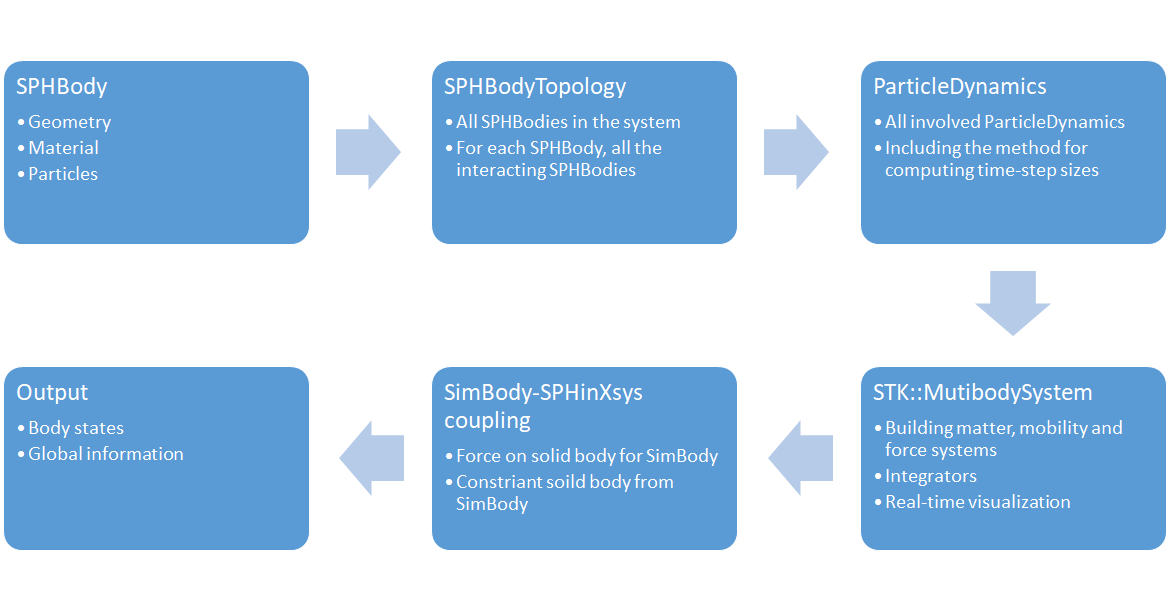
\includegraphics[width=\textwidth]{figs/initialization.png}
	\caption{Constructing a computation with ordered stages. }
	\label{figs:construction}
\end{figure}
%
At the second stage, the topology of \texttt{SPHBody}s is constructed. 
It describe, for each \texttt{SPHBody}, all the interacting \texttt{SPHBody}s. 
After this, all \texttt{ParticleDynamics} will be defined.
Specifically, each realization of \texttt{ParticleDynamics} 
corresponds all the discretized right-hand-side terms of a fluid or solid dynamics equation.
If SPHinXsys is coupled with SimBody, one need create a \texttt{SimTK} system in which all matters, mobility and forces are defined. The SimBody-SPHinXsys coupling, 
as a realization of \texttt{ParticleDynamics}, 
such as computing forces on solid body for SimBody 
and imposing constriants of soild body by SimBody, are defined in the next stage.
Finally, \texttt{Output} is created to specify the data will be saved in file during the computations.
%
\subsubsection{Carrying out a computation}
The computation is carried out by using an integrator defined in the application.
There are three layers in the main integration step according to their the time-step sizes.
While at the innermost layer the solid dynamics equations are integrated, 
at the middle layer the acoustic pressure relaxation of the fluid is computed 
and at the outside layer the effects of fluid viscosity is updated.
The FSI is imposed at the middle layer 
and the coupling with Simbody is implemented at the innermost layer.
%
\newpage
\section{Installing SPHinXsys}\label{install}
This section describes the installation procedure for the precompiled binaries of the SPHinXsys. 
If you want to build from source instead, please see the separate document ―How to Build Simbody from Source. 
That document is included in the source zip file.
\subsection{General instruction}
\subsubsection{General instructions}
We’ll start here with general information, then give platform-specific instructions in sections \ref{install-unix} (Linux and Mac OX S), and \ref{install-win} (Windows).
Be sure to check the online installation instructions that are alongside the download package for last-minute information.
\subsubsection{Where can I find the downloads}
Access is granted on request via email: xiangyu.hu@tum.de
\subsubsection{What is in the download zip files}
The downloads include libraries, header files, documentation and example programs for SPHinXsys. 
The installation is organized as a hierarchy of directories. 
The top level directory has 5 subdirectories: lib, include, doc, and case test. 
The downloads contain static and dynamic versions of each library, in both debug and optimized form. 
All the examples are available precompiled, and source and build scripts for them are in examples/src. 
\subsubsection{Which download do I want}
There are separate download packages for each of the supported platforms (Linux, Mac OS X, and Windows).
There is also a source package but if you want to build from source you are reading the wrong document – see above.
\subsubsection{What if I have a problem}
If you have problems, e.g., bug report and contribute to the development of SPHinXsys, 
please email to xiangyu.hu@tum.de (Xiangyu Hu) or c.zhang@tum.de (Chi Zhang).
\subsubsection{Installation overview}
Here is the general procedure
\begin{itemize}
	\item Set up your machine with the required prerequisites.
	\item Download the appropriate .zip package from the Downloads page.
	\item  Unzip into the installation directory (can be anywhere but we’ll suggest default locations).
	\item  Set path and environment variables as needed.
	\item  Run installation test programs to verify.
	\item SimBody library 3.6.0 or higher.
\end{itemize}
The next three sections provided details specific to each of the three platforms for which we provide binaries: Linux, Mac, Windows. You only need to read one of these sections.
\subsection{Dependencies}
SPHinXsys depends on the following:
\begin{itemize}
	\item  cross-platform building: Cmake 3.14.0 or later. see \url{https://cmake.org/}
	\item compiler: Visual Studio 2017 (Windows only), gcc 4.9 or later (typically on Linux), or Apple Clang (1001.0.46.3)  or later
	\item BOOST library (newest version)
	\item TBB library (newest version)
	\item Simbody library 3.6.0 or later
	\item linear algebra: LAPACK 3.5.0 or later and BLAS
\end{itemize}
\subsection{Installing on Unix(Linux or Mac OS X)}\label{install-unix}
The only prerequisite on Mac OS X is that you have the developer kit installed, 
which you probably do already.
At a minimum, the Accelerate framework must be installed 
because that includes Lapack ad Blas libraries on which Simbody depends. 
If you download the developer kit, those libraries are installed as well.

On Linux system, LAPACK and BLAS is require, and we refer to \url{http://www.netlib.org/lapack/} and \url{http://www.netlib.org/blas/} for more details.

The installation of Simbody, refers to \url{https://github.com/simbody/simbody#linux-or-mac-using-make }.
After installing Simbody correctly, set environment variable:
\begin{itemize}
\item  For Mac OS X
\begin{lstlisting}[language=Bash]
$ echo 'export TBB_HOME=/path/to/tbb' >> ~/.bash_profile
\end{lstlisting}
\item  For Linux
\begin{lstlisting}[language=Bash]
$ echo 'export TBB_HOME=/path/to/tbb' >> ~/.bashrc
$ echo 'export LIBRARY_PATH=$SIMBODY_HOME/lib64:$LIBRARY_PATH' >> ~/.bashrc
$ echo 'export LD_LIBRARY_PATH=$LIBRARY_PATH:$LD_LIBRARY_PATH' >> ~/.bashrc
$ echo 'export CPLUS_INCLUDE_PATH=$SIMBODY_HOME/include:$CPLUS_INCLUDE_PATH' << ~/.bashrc
\end{lstlisting} 
\end{itemize}

Download a release version of TBB from \url{https://github.com/01org/tbb/releases} and then unzip it to the appropriate directory on your computer and set environment variable:
\begin{itemize}
\item Mac OS X
\begin{lstlisting}[language=Bash]
$ echo 'export TBB_HOME=/path/to/tbb' >> ~/.bash_profile
\end{lstlisting}
\item Linux
\begin{lstlisting}[language=Bash]
$ echo 'export TBB_HOME=/path/to/tbb' >> ~/.bashrc
\end{lstlisting}
\end{itemize}
Download a release version of BOOST from :\url{https://www.boost.org/users/download/} and then unzip it to the appropriate directory on your computer and set environment variable:
\begin{itemize}
\item Mac OS X
\begin{lstlisting}[language=Bash]
$ echo 'export BOOST_HOME=/path/to/boost' >> ~/.bash_profile
\end{lstlisting}
\item  Linux
\begin{lstlisting}[language=Bash]
$ echo 'export BOOST_HOME=/path/to/boost' >> ~/.bashrc
\end{lstlisting}
\end{itemize}

Download the sphinxsys-linux or sphinxsys-max, and then unzip it to the appropriate directory on your computer and set environment variable \begin{itemize}
	\item Mac OS X
\begin{lstlisting}[language=Bash]
$ echo 'export SPHINXSYS_HOME=/path/to/sphinxsyslibaray' >> ~/.bash_profile
\end{lstlisting}
\item  Linux
\begin{lstlisting}[language=Bash]
$ echo 'export SPHINXSYS_HOME=/path/to/sphinxsyslibrary' >> ~/.bashrc
\end{lstlisting}
\end{itemize}
and then using the following commend to build the SPHINXSYS and run with the following command:
\begin{lstlisting}[language=Bash]
$  cmake /path/to/sphinxsys-alpha -DCMAKE_INSTALL_PREFIX=/path/to/sphinxsys-prefix -DCMAKE_BUILD_TYPE=RelWithDebInfo
$ cd example
$ make -j
$ cd bin/
$ ./example
\end{lstlisting}
Right now, you can play with SPHinXsys by change the parameters. GOOD LUCK!
\subsection{Installing on Windows}\label{install-win}
We provide pre-built binaries for use with Visual Studio 2017. 
If you have an earlier or later version of Visual Studio, or if you are using Visual Studio Express you will likely need to build from source (not hard). See the separate build from source document referenced at the start of this chapter.

The only prerequisite on Windows is that you have a development environment (Visual Studio) and a way to unzip the .zip package. If you don’t have one already, you’ll need to install software that can perform the unzip operation. 
The installation of Simbody on Windows is refer to \url{https://github.com/simbody/simbody#windows-using-visual-studio}, 
and after that please set the system environment variable SIMBODY\_HOME to the simbody prefix directory and the simbody bin path  to environmental variable( System variable)

Install TBB, actually extract the file to the assigned folder , e.g. $C:/ tbb\_2019$
set environment variable: TBB\_HOME to the tbb directory, and set the path $path/to/tbbe/bin/intel64/vc14$ to environmental variable (System variables).

Install boost, actually extract the file to the assigned folder, e,g, C:/boost, and set environment: BOOST\_HOME to its directory

Download the sphinxsys-win file,
and then unzip it to the appropriate directory on your computer and set environment variable BOOST\_HOME to its directory.
Using cmake for configure project as follows 
%
\begin{figure}[tb!]
	\centering
	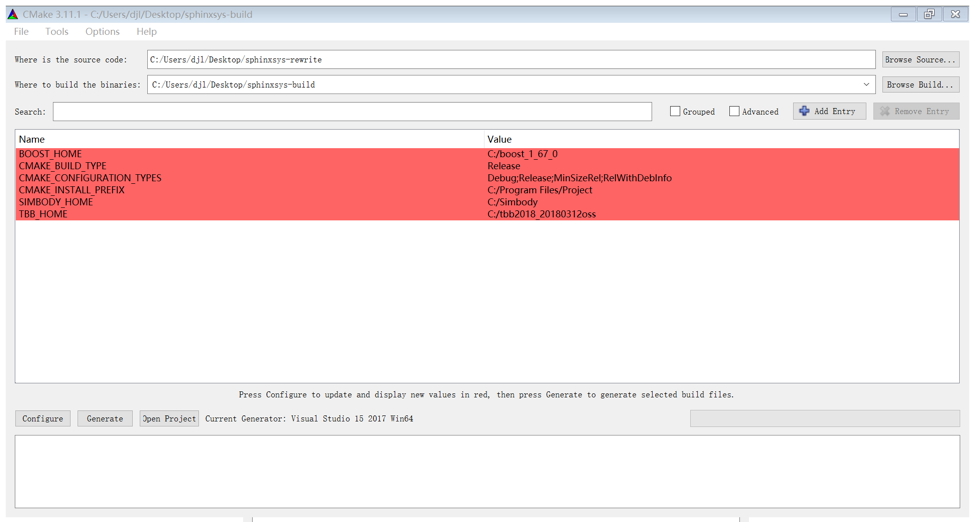
\includegraphics[width=\textwidth]{figs/cmake-sphinxsys.png}
	\caption{Cmake configure sphinxsys library. }
	\label{figs:win-sphinxsys}
\end{figure}
%
After configuration, one can use Visual Studio to play with SPHinXsys. GOOD LUCK!

\section{Simple Example: 2D Dam break}\label{example}
It’s now time to look at our first example. 
Here we’ll introduce features as we go. In the next chapter we’ll step back and talk more about the SPHinXsys applications in general.
%
\subsection{A First Example}
The following program creates a system for the dam break problem: 
a water block is released and moves under 
the action of gravity within a water tank.
It simulates the behavior of this system over a time interval 
in which the water wave impacts the tank wall and producing splashes.
%
\begin{lstlisting}[basicstyle=\ttfamily\footnotesize]
/**
* @file 	Dambreak.cpp
* @brief 	2D dambreak exaple.
* @details This is the one of the basic test cases, also the first case for
* 			understanding SPH method for fluid similation.
* @author 	Luhui Han, Chi Zhang and Xiangyu Hu
* @version 0.1
*/
/**
* @brief SPHinXsys Library.
*/
#include "sphinxsys.h"
/**
* @brief Namespace cite here.
*/
using namespace SPH;
/**
* @brief Basic geometry parameters and numerical setup.
*/
Real DL = 5.366; 						/**< Tank length. */
Real DH = 5.366; 						/**< Tank height. */
Real LL = 2.0; 							/**< Liquid colume length. */
Real LH = 1.0; 							/**< Liquid colume height. */
Real particle_spacing_ref = 0.025; 		/**< Initial reference particle spacing. */
Real BW = particle_spacing_ref * 4; 	/**< Extending width for BCs. */
/**
* @brief Material properties of the fluid.
*/
Real rho0_f = 1.0;						/**< Reference density of fluid. */
Real gravity_g = 1.0;					/**< Gravity force of fluid. */
Real U_f = 2.0*sqrt(gravity_g*LH);		/**< Characteristic velocity. */
Real c_f = 10.0*U_f;					/**< Reference sound speed. */

Real initial_pressure = 0.0;			/**< Initial pressure field. */
Vec2d intial_velocity(0.0, 0.0);		/**< Initial velocity field. */
/**
* @brief 	Fluid body definition.
*/
class WaterBlock : public WeaklyCompressibleFluidBody
{
public:
	WaterBlock(SPHSystem &system, string body_name,
	WeaklyCompressibleFluid* material,
	WeaklyCompressibleFluidParticles
	&weakly_compressible_fluid_particles, int refinement_level, ParticlesGeneratorOps op)
	: WeaklyCompressibleFluidBody(system, body_name, material,
		weakly_compressible_fluid_particles, refinement_level, op)
	{
		/** Geomerty definition. */
		std::vector<Point> water_block_shape;
		water_block_shape.push_back(Point(0.0, 0.0));
		water_block_shape.push_back(Point(0.0, LH));
		water_block_shape.push_back(Point(LL, LH));
		water_block_shape.push_back(Point(LL, 0.0));
		water_block_shape.push_back(Point(0.0, 0.0));
		Geometry *water_block_geometry = new Geometry(water_block_shape);
		body_region_.add_geometry(water_block_geometry, RegionBooleanOps::add);

		body_region_.done_modeling();
	}
	/** Initialize every fluid particle data. */
	void InitialCondition()
	{
		for (int i = 0; i < number_of_particles_; ++i) {
			BaseParticleData  &base_particle_data_i = weakly_compressible_fluid_particles_.base_particle_data_[i];
			WeaklyCompressibleFluidParticleData 
				&fluid_data_i
				= weakly_compressible_fluid_particles_.fluid_data_[i];

			fluid_data_i.p_ = initial_pressure;
			base_particle_data_i.vel_n_ = intial_velocity;
			base_particle_data_i.dvel_dt_(0);
			fluid_data_i.rho_0_
				= material_->ReinitializeRho(initial_pressure);
			fluid_data_i.rho_n_ = fluid_data_i.rho_0_;
			fluid_data_i.mass_
				= fluid_data_i.rho_0_*base_particle_data_i.Vol_;
		}
	}
};
/**
* @brief 	Wall boundary body definition.
*/
class WallBoundary : public SolidBody
{
public:
	WallBoundary(SPHSystem &system, string body_name,
		SolidBodyParticles &solid_particles, int refinement_level, ParticlesGeneratorOps op)
		: SolidBody(system, body_name, solid_particles, refinement_level, op)
	{
		/** Geomerty definition. */
		std::vector<Point> outer_wall_shape;
		outer_wall_shape.push_back(Point(-BW, -BW));
		outer_wall_shape.push_back(Point(-BW, DH + BW));
		outer_wall_shape.push_back(Point(DL + BW, DH + BW));
		outer_wall_shape.push_back(Point(DL + BW, -BW));
		outer_wall_shape.push_back(Point(-BW, -BW));
		Geometry *outer_wall_geometry = new Geometry(outer_wall_shape);
		body_region_.add_geometry(outer_wall_geometry, RegionBooleanOps::add);

		std::vector<Point> inner_wall_shape;
		inner_wall_shape.push_back(Point(0.0, 0.0));
		inner_wall_shape.push_back(Point(0.0, DH));
		inner_wall_shape.push_back(Point(DL, DH));
		inner_wall_shape.push_back(Point(DL, 0.0));
		inner_wall_shape.push_back(Point(0.0, 0.0));
		Geometry *inner_wall_geometry = new Geometry(inner_wall_shape);
		body_region_.add_geometry(inner_wall_geometry, RegionBooleanOps::sub);

		body_region_.done_modeling();
	}
	/** Initialize every wallboundary particle data. */
	void InitialCondition()
	{
		for (int i = 0; i < solid_particles_.number_of_particles_; ++i) {
			BaseParticleData &base_particle_data_i
				= solid_particles_.base_particle_data_[i];
			SolidBodyParticleData &solid_body_data_i
				= solid_particles_.solid_body_data_[i];
	
			base_particle_data_i.vel_n_ = intial_velocity;
			Vec2d zero(0);
			base_particle_data_i.dvel_dt_ = zero;
			solid_body_data_i.vel_ave_ = zero;
			solid_body_data_i.dvel_dt_ave_ = zero;
		}
	}
};
/**
* @brief 	Fluid observer body definition.
*/
class FluidObserver : public ObserverBody
{
public:
	FluidObserver(SPHSystem &system, string body_name,
		ObserverParticles &observer_particles, int refinement_level, ParticlesGeneratorOps op)
		: ObserverBody(system, body_name, observer_particles, refinement_level, op)
	{
		body_input_points_volumes_.push_back(make_pair(Point(DL, 0.2), 0.0));
	}
};
/**
* @brief 	Main program starts here.
*/
int main()
{
	/**
	* @brief Build up -- a SPHSystem --
	*/
	SPHSystem system(Vec2d(-BW, -BW), Vec2d(DL + BW, DH + BW), particle_spacing_ref);
	/** Set the starting time. */
	GlobalStaticVariables::physical_time_ = 0.0;
	/** Tag for computation from restart files. 0: not from restart files. */
	system.restart_step_ = 0;
	/**
	* @brief Material property, partilces and body creation of fluid.
	*/
	WeaklyCompressibleFluid 			fluid("Water", rho0_f, c_f, mu_f, k_f);
	WeaklyCompressibleFluidParticles 	fluid_particles("WaterBody");
	WaterBlock *water_block = new WaterBlock(system, "WaterBody", &fluid,
		fluid_particles, 0, ParticlesGeneratorOps::lattice);
	/**
	* @brief 	Particle and body creation of wall boundary.
	*/
	SolidBodyParticles 					solid_particles("Wall");
	WallBoundary *wall_boundary = new WallBoundary(system, "Wall",
		solid_particles, 0, ParticlesGeneratorOps::lattice);
	/**
	* @brief 	Particle and body creation of fluid observer.
	*/
	ObserverParticles 					observer_particles("Fluidobserver");
	FluidObserver *fluid_observer = new FluidObserver(system, "Fluidobserver",
		observer_particles, 0, ParticlesGeneratorOps::direct);
	/**
	* @brief 	Body contact map.
	* @details The contact map gives the data conntections between the bodies.
	* 			Basically the the rang of bidies to build neighbor particle lists.
	*/
	SPHBodyTopology 	body_topology = { { water_block, { wall_boundary } },
											{ wall_boundary, {} },{ fluid_observer,{ water_block} } };
	system.SetBodyTopology(&body_topology);
	/**
	* @brief 	Simulation set up.
	*/
	system.SetupSPHSimulation();
	/**
	* @brief 	Define all numerical methods which are used in this case.
	*/
	/** Define external force. */
	Gravity 							gravity(Vecd(0.0, -gravity_g));
	/**
	* @brief 	Methods used only once.
	*/
	/** Initialize normal direction of the wall boundary. */
	solid_dynamics::NormalDirectionSummation 	get_wall_normal(wall_boundary, {});
	get_wall_normal.exec();
	/** Obtain the initial number density of fluid. */
	fluid_dynamics::InitialNumberDensity 		
		fluid_initial_number_density(water_block, { wall_boundary });
	fluid_initial_number_density.exec();
	/**
	* @brief 	Methods used for time stepping.
	*/
	/** Initialize particle acceleration. */
	InitializeOtherAccelerations 	initialize_fluid_acceleration(water_block);
	/** Add particle acceleration due to gravity force. */
	AddGravityAcceleration 			add_fluid_gravity(water_block, &gravity);
	/**
	* @brief 	Algorithms of fluid dynamics.
	*/
	/** Wvaluation of density by summation approach. */
	fluid_dynamics::DensityBySummationFreeSurface 		
		update_fluid_desnity(water_block, { wall_boundary });
	/** Time step size without considering sound wave speed. */
	fluid_dynamics::FluidAdvectionTimeStepSize 			
		get_fluid_adevction_time_step_size(water_block, U_f);
	/** Time step size with considering sound wave speed. */
	fluid_dynamics::WeaklyCompressibleFluidTimeStepSize get_fluid_time_step_size(water_block);
	/** Pressure relaxation algorithm by using verlet time stepping. */
	fluid_dynamics::PressureRelaxationVerletFreeSurface 
		pressure_relaxation(water_block, { wall_boundary }, &gravity);
	/**
	* @brief 	Methods used for updating data structure.
	*/
	/** Update the cell linked list of bodies when neccessary. */
	ParticleDynamicsCellLinkedList			update_cell_linked_list(water_block);
	/** Update the configuration of bodies when neccessary. */
	ParticleDynamicsConfiguration 			update_particle_configuration(water_block);
	/** Update the interact configuration of bodies when neccessary. */
	ParticleDynamicsInteractionConfiguration 	
		update_observer_interact_configuration(fluid_observer, { water_block });
	/**
	* @brief Output.
	*/
	Output output(system);
	/** Output the body states. */
	WriteBodyStatesToVtu 		write_body_states(output, system.real_bodies_);
	/** Output the body states for restart simulation. */
	WriteRestartFileToXml		write_restart_body_states(output, system.real_bodies_);
	/** Output the mechanical energy of fluid body. */
	WriteWaterMechanicalEnergy 	write_water_mechanical_energy(output, water_block, &gravity);
	/** output the observed data from fluid body. */
	WriteObservedFluidPressure	write_recorded_water_pressure(output, fluid_observer, { water_block });
	/**
	* @brief The time stepping starts here.
	*/
	/** If the starting time is not zero, please setup the restart time step ro read in restart states. */
	if (system.restart_step_ != 0)
	{
		system.ResetSPHSimulationFromRestart();
		update_cell_linked_list.parallel_exec();
		update_particle_configuration.parallel_exec();
	}
	/** Output the start states of bodies. */
	write_body_states
		.WriteToFile(GlobalStaticVariables::physical_time_);
	/** Output the Hydrostatic mechanical energy of fluid. */
	write_water_mechanical_energy
		.WriteToFile(GlobalStaticVariables::physical_time_);
	/**
	* @brief 	Basic parameters.
	*/
	int ite = system.restart_step_;
	int rst_out = 1000;
	Real End_Time = 20.0; 	/**< End time. */
	Real D_Time = 0.1;		/**< Time stamps for output of body states. */
	Real Dt = 0.0;			/**< Default advection time step sizes. */
	Real dt = 0.0; 			/**< Default accoustic time step sizes. */
	/** statistics for computing CPU time. */
	tick_count t1 = tick_count::now();
	tick_count::interval_t interval;
	/** Output global basic parameters. */
	output.WriteCaseSetup(End_Time, D_Time, GlobalStaticVariables::physical_time_);
	/**
	* @brief 	Main loop starts here.
	*/
	while (GlobalStaticVariables::physical_time_ < End_Time)
	{
			Real integeral_time = 0.0;
			/** Integrate time (loop) until the next output time. */
			while (integeral_time < D_Time)
			{
				/** Acceleration due to viscous force and gravity. */
				initialize_fluid_acceleration.parallel_exec();
				add_fluid_gravity.parallel_exec();
				Dt = get_fluid_adevction_time_step_size.parallel_exec();
				update_fluid_desnity.parallel_exec();
				
				/** Dynamics including pressure relaxation. */
				Real relaxation_time = 0.0;
				while (relaxation_time < Dt)
				{
					if (ite % 100 == 0)
					{
						cout << "N=" << ite << " Time: "
						<< GlobalStaticVariables::physical_time_
						<< "	dt: " << dt << "\n";
						if (ite % rst_out == 0)
						write_restart_body_states.WriteToFile(Real(ite));
					}
					pressure_relaxation.parallel_exec(dt);
					
					ite++;
					dt = get_fluid_time_step_size.parallel_exec();
					relaxation_time += dt;
					integeral_time += dt;
					GlobalStaticVariables::physical_time_ += dt;
				
				}
				/** Update cell linked list and configuration. */
				update_cell_linked_list.parallel_exec();
				update_particle_configuration.parallel_exec();
				update_observer_interact_configuration.parallel_exec();
			}
			
			tick_count t2 = tick_count::now();
			write_water_mechanical_energy
				.WriteToFile(GlobalStaticVariables::physical_time_);
			write_body_states
				.WriteToFile(GlobalStaticVariables::physical_time_);
			write_recorded_water_pressure
				.WriteToFile(GlobalStaticVariables::physical_time_);
			tick_count t3 = tick_count::now();
			interval += t3 - t2;
		}
	tick_count t4 = tick_count::now();
	
	tick_count::interval_t tt;
	tt = t4 - t1 - interval;
	cout << "Total wall time for computation: " << tt.seconds()
	<< " seconds." << endl;
	
	return 0;
}

\end{lstlisting}
%
Before you can compile and run this program, 
you need to have SPHinXsys installed (see Chapter \ref{install}). 
The installation directory has subdirectories \texttt{include}, \texttt{lib}, and \texttt{bin}. 
Make sure the \texttt{include} directory is part of your compiler’s include path, and the \texttt{lib} directory is available to the linker. At runtime the shared library directory (lib for Mac and Linux, bin for Windows) must be on the appropriate  \texttt{path} environment variable. Exactly how you do this will depend on the compiler and operating system you are using.

If everything is working correctly, 
you should see a new folder \texttt{output} is created and particle state files start with \texttt{SPHBody}
and \texttt{Fluidobserver\_fluid\_pressure.dat} and \texttt{WaterBody\_water\_mechnical\_energy.dat}, 
which are global information files.
In the visualization software Paraview you can produces the particle distribution as shown in Fig \ref{figs:dambreak}. 
%
\begin{figure}[tb!]
	\centering
	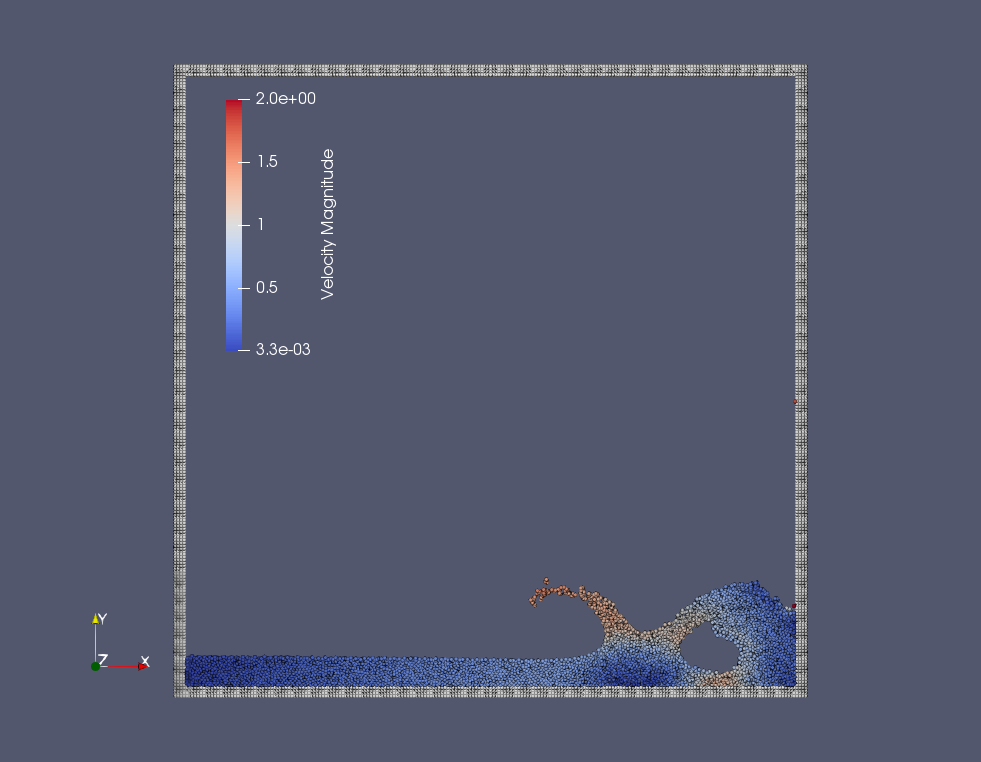
\includegraphics[width=\textwidth]{figs/dambreak.png}
	\caption{A snapshot of the particle distribution in the dam break problem.}
	\label{figs:dambreak}
\end{figure}
%
Let’s go through the program line by line and see how it works. 
It begins with the include statements:
%
\begin{lstlisting}[basicstyle=\ttfamily\footnotesize]
/**
* @file 	Dambreak.cpp
* @brief 	2D dambreak exaple.
* @details This is the one of the basic test cases, also the first case for
* 			understanding SPH method for fluid similation.
* @author 	Luhui Han, Chi Zhang and Xiangyu Hu
* @version 0.1
*/
/**
* @brief SPHinXsys Library.
*/
#include "sphinxsys.h"
\end{lstlisting}
%
That gets us all the declarations we need to write a SPHinXsys-using application.

Next we import the \texttt{SPH} namespace, 
which includes nearly all of the symbols used by SPHinXsys:
%
\begin{lstlisting}[basicstyle=\ttfamily\footnotesize]
/**
* @brief Namespace cite here.
*/
using namespace SPH;
\end{lstlisting}
%

Now, we provide the parameters for geometric modeling.
%
\begin{lstlisting}[basicstyle=\ttfamily\footnotesize]
/**
* @brief Basic geometry parameters and numerical setup.
*/
Real DL = 5.366; 						/**< Tank length. */
Real DH = 5.366; 						/**< Tank height. */
Real LL = 2.0; 							/**< Liquid colume length. */
Real LH = 1.0; 							/**< Liquid colume height. */
Real particle_spacing_ref = 0.025; 		/**< Initial reference particle spacing. */
Real BW = particle_spacing_ref * 4; 	/**< Extending width for BCs. */
\end{lstlisting}
%
Here, \texttt{particle\_spacing\_ref} gives 
the reference initial particle spacing for multi-resolution modeling, e.g. for refinement level 0. 
\texttt{BW} is the size (thickness) of a wall boundary, which is usually 4 times of particle spacing.

We also provide parameters for physical modeling, 
such as material properties of the fluid and physical parameters of the dam break problem.
%
\begin{lstlisting}[basicstyle=\ttfamily\footnotesize]
/**
* @brief Material properties of the fluid.
*/
Real rho0_f = 1.0;						/**< Reference density of fluid. */
Real gravity_g = 1.0;					/**< Gravity force of fluid. */
Real U_f = 2.0*sqrt(gravity_g*LH);		/**< Characteristic velocity. */
Real c_f = 10.0*U_f;					/**< Reference sound speed. */

Real initial_pressure = 0.0;			/**< Initial pressure field. */
Vec2d intial_velocity(0.0, 0.0);		/**< Initial velocity field. */
\end{lstlisting}
%
As we are using a weakly compressible model for imposing incompressibility, 
the maximum speed in the flow and artificial speed of sound are estimated.

Then, we define the realization of \texttt{SPHBody}s. 
First, a \texttt{WaterBlock}, which is a derived class of \texttt{WeaklyCompressibleFluidBody}, 
is defined with constructor parameters, such as material, particles, refinement level 
and the option for particle generator.
%
\begin{lstlisting}[basicstyle=\ttfamily\footnotesize]
/**
* @brief 	Fluid body definition.
*/
class WaterBlock : public WeaklyCompressibleFluidBody
{
	public:
	WaterBlock(SPHSystem &system, string body_name,
		WeaklyCompressibleFluid* material,
		WeaklyCompressibleFluidParticles
		&weakly_compressible_fluid_particles, int refinement_level, ParticlesGeneratorOps op)
		: WeaklyCompressibleFluidBody(system, body_name, material,
		weakly_compressible_fluid_particles, refinement_level, op)
	{
		/** Geomerty definition. */
		std::vector<Point> water_block_shape;
		water_block_shape.push_back(Point(0.0, 0.0));
		water_block_shape.push_back(Point(0.0, LH));
		water_block_shape.push_back(Point(LL, LH));
		water_block_shape.push_back(Point(LL, 0.0));
		water_block_shape.push_back(Point(0.0, 0.0));
		Geometry *water_block_geometry = new Geometry(water_block_shape);
		body_region_.add_geometry(water_block_geometry, RegionBooleanOps::add);
		
		body_region_.done_modeling();
	}
	/** Initialize every fluid particle data. */
	void InitialCondition()
	{
		for (int i = 0; i < number_of_particles_; ++i) {
			BaseParticleData &base_particle_data_i
				= weakly_compressible_fluid_particles_.base_particle_data_[i];
			WeaklyCompressibleFluidParticleData &fluid_data_i
				= weakly_compressible_fluid_particles_.fluid_data_[i];
			
			fluid_data_i.p_ = initial_pressure;
			base_particle_data_i.vel_n_ = intial_velocity;
			base_particle_data_i.dvel_dt_(0);
			fluid_data_i.rho_0_
				= material_->ReinitializeRho(initial_pressure);
			fluid_data_i.rho_n_ = fluid_data_i.rho_0_;
			fluid_data_i.mass_
				= fluid_data_i.rho_0_*base_particle_data_i.Vol_;
		}
	}
};
\end{lstlisting}
%
Here, the body geometry is defined from the coordinates 
based on the geometric parameters and binary operations, 
such as \texttt{add} and \texttt{sub}.
Note that, the initial condition of the \texttt{WaterBlock} 
is also given in a member function \texttt{void InitialCondition()}.
Similarly, we define the \texttt{WallBoundary} and \texttt{FluidObserver}.
Note that there is no initial condition for the observation body
as it usually only obtain data from the body it is observing at.

After all \texttt{SPHBody}s are defined, here comes to the \texttt{int main()} function,
which the application is defined.
In the first part of \texttt{main} function, 
an object of \texttt{SPHSystem} is created, global physical time initialized,
and whether the computation begin from restart files is checked.
%
\begin{lstlisting}[basicstyle=\ttfamily\footnotesize]
/**
* @brief Build up -- a SPHSystem --
*/
SPHSystem system(Vec2d(-BW, -BW), Vec2d(DL + BW, DH + BW), particle_spacing_ref);
/** Set the starting time. */
GlobalStaticVariables::physical_time_ = 0.0;
/** Tag for computation from restart files. 0: not from restart files. */
system.restart_step_ = 0;
/**
* @brief Material property, partilces and body creation of fluid.
*/
WeaklyCompressibleFluid 			fluid("Water", rho0_f, c_f, mu_f, k_f);
WeaklyCompressibleFluidParticles 	fluid_particles("WaterBody");
WaterBlock *water_block = new WaterBlock(system, "WaterBody", 
	&fluid, fluid_particles, 0, ParticlesGeneratorOps::lattice);
/**
* @brief 	Particle and body creation of wall boundary.
*/
SolidBodyParticles 					solid_particles("Wall");
WallBoundary *wall_boundary = new WallBoundary(system, "Wall",
solid_particles, 0, ParticlesGeneratorOps::lattice);
/**
* @brief 	Particle and body creation of fluid observer.
*/
ObserverParticles 					observer_particles("Fluidobserver");
FluidObserver *fluid_observer = new FluidObserver(system, "Fluidobserver",
observer_particles, 0, ParticlesGeneratorOps::direct);
/**
* @brief 	Body contact map.
* @details The contact map gives the data conntections between the bodies.
* 			Basically the the rang of bidies to build neighbor particle lists.
*/
SPHBodyTopology 	body_topology = { { water_block, { wall_boundary } },
{ wall_boundary, {} },{ fluid_observer,{ water_block} } };
system.SetBodyTopology(&body_topology);
/**
* @brief 	Simulation set up.
*/
system.SetupSPHSimulation();
\end{lstlisting}
%
Note that the constructor of \texttt{SPHSystem} requires the coordinates of 
lower and upper bounds of the domain, which will be used as the bounds 
for a mesh used for building cell linked lists.
The material, particles and bodies are also created for water block, wall and observer. 
Then, the collection of topological relations,
which specifies for each body the possible interacting bodies, 
are defined. The function \texttt{SetupSPHSimulation()} creates SPH particles,
builds particle configurations and set initial condition if necessary.

After this, the physical dynamics of system is defined 
as method classes in the form of particle discretization.
%
\begin{lstlisting}[basicstyle=\ttfamily\footnotesize]
	/**
* @brief 	Define all numerical methods which are used in this case.
*/
/** Define external force. */
Gravity 							gravity(Vecd(0.0, -gravity_g));
/**
* @brief 	Methods used only once.
*/
/** Initialize normal direction of the wall boundary. */
solid_dynamics::NormalDirectionSummation 	get_wall_normal(wall_boundary, {});
get_wall_normal.exec();
/** Obtain the initial number density of fluid. */
fluid_dynamics::InitialNumberDensity 		
fluid_initial_number_density(water_block, { wall_boundary });
fluid_initial_number_density.exec();
/**
* @brief 	Methods used for time stepping.
*/
/** Initialize particle acceleration. */
InitializeOtherAccelerations 	initialize_fluid_acceleration(water_block);
/** Add particle acceleration due to gravity force. */
AddGravityAcceleration 			add_fluid_gravity(water_block, &gravity);
/**
* @brief 	Algorithms of fluid dynamics.
*/
/** Wvaluation of density by summation approach. */
fluid_dynamics::DensityBySummationFreeSurface 		
update_fluid_desnity(water_block, { wall_boundary });
/** Time step size without considering sound wave speed. */
fluid_dynamics::FluidAdvectionTimeStepSize 			
get_fluid_adevction_time_step_size(water_block, U_f);
/** Time step size with considering sound wave speed. */
fluid_dynamics::WeaklyCompressibleFluidTimeStepSize get_fluid_time_step_size(water_block);
/** Pressure relaxation algorithm by using verlet time stepping. */
fluid_dynamics::PressureRelaxationVerletFreeSurface 
pressure_relaxation(water_block, { wall_boundary }, &gravity);
\end{lstlisting}
%
First, the external force is defined.
Then comes the methods that will be used only once,
such as computing normal direction of the static wall surface, 
and  the initial particle number density. 
Then, the methods that will used for multiple times are defined.
They are the SPH algorithms for fluid dynamics, time step criteria.

The methods for updating particle configurations will be realized in the following,
including update cell linked list, inner (within the body) 
and contact (with the interacting bodies) neighboring particles.
%
\begin{lstlisting}[basicstyle=\ttfamily\footnotesize]
/**
* @brief 	Methods used for updating data structure.
*/
/** Update the cell linked list of bodies when neccessary. */
ParticleDynamicsCellLinkedList			update_cell_linked_list(water_block);
/** Update the configuration of bodies when neccessary. */
ParticleDynamicsConfiguration 			update_particle_configuration(water_block);
/** Update the interact configuration of bodies when neccessary. */
ParticleDynamicsInteractionConfiguration 	
	update_observer_interact_configuration(fluid_observer, { water_block });
\end{lstlisting}
%
Note that such updating can be specified for a given body for its inner and/or 
all contact configuration or cell-linked list, 
or given pair of bodies for the interact configuration.

Before the computation, we also define the outputs, 
including the particle states, restart files, global values and observations.
%
\begin{lstlisting}[basicstyle=\ttfamily\footnotesize]
	/**
* @brief Output.
*/
Output output(system);
/** Output the body states. */
WriteBodyStatesToVtu 		write_body_states(output, system.real_bodies_);
/** Output the body states for restart simulation. */
WriteRestartFileToXml		write_restart_body_states(output, system.real_bodies_);
/** Output the mechanical energy of fluid body. */
WriteWaterMechanicalEnergy 	write_water_mechanical_energy(output, water_block, &gravity);
/** output the observed data from fluid body. */
WriteObservedFluidPressure	write_recorded_water_pressure(output, fluid_observer, { water_block });\end{lstlisting}
%
The \texttt{Vtu} files can be read directly by the open-source visualization code ParaView.
You also have the option to save the files in Tecplot format.
The global information and observation data are written in simple data format. 
The restart files are in \texttt{XML} data format.

Finally, the time stepping will almost start. 
However, if the computation begin from restart files. 
The system will be reset.  
%
\begin{lstlisting}[basicstyle=\ttfamily\footnotesize]
	/**
* @brief The time stepping starts here.
*/
/** If the starting time is not zero, please setup the restart time step ro read in restart states. */
if (system.restart_step_ != 0)
{
	system.ResetSPHSimulationFromRestart();
	update_cell_linked_list.parallel_exec();
	update_particle_configuration.parallel_exec();
}
/** Output the start states of bodies. */
write_body_states.WriteToFile(GlobalStaticVariables::physical_time_);
/** Output the Hydrostatic mechanical energy of fluid. */
write_water_mechanical_energy.WriteToFile(GlobalStaticVariables::physical_time_);
\end{lstlisting}
%
Note that, because the particles have been moved in the previous simulation, 
one need to update the cell-linked list and particle configuration. 
After that, the states from the starting time step will be outputted. 

The basic control parameter for the simulation is defined.
Such as the restart file output frequency, total simulation time 
and interval for writing output files. 
%
\begin{lstlisting}[basicstyle=\ttfamily\footnotesize]
	/**
* @brief 	Basic parameters.
*/
int ite = system.restart_step_;
int rst_out = 1000;
Real End_Time = 20.0; 	/**< End time. */
Real D_Time = 0.1;		/**< Time stamps for output of body states. */
Real Dt = 0.0;			/**< Default advection time step sizes. */
Real dt = 0.0; 			/**< Default accoustic time step sizes. */
/** statistics for computing CPU time. */
tick_count t1 = tick_count::now();
tick_count::interval_t interval;
/** Output global basic parameters. */
output.WriteCaseSetup(End_Time, D_Time, GlobalStaticVariables::physical_time_);
\end{lstlisting}
%
Also the statistic for computation time is initialized.
A case setup file will be written as a summary of the case. This file goes together with other output data for later reference.

Here comes the time-stepping loops. 
The computation is carried out with a dual-criteria time-stepping scheme,
as discussed in Chapter \ref{theory}.
%
\begin{lstlisting}[basicstyle=\ttfamily\footnotesize]
	/**
* @brief 	Main loop starts here.
*/
while (GlobalStaticVariables::physical_time_ < End_Time)
{
	Real integeral_time = 0.0;
	/** Integrate time (loop) until the next output time. */
	while (integeral_time < D_Time)
	{
		/** Acceleration due to viscous force and gravity. */
		initialize_fluid_acceleration.parallel_exec();
		add_fluid_gravity.parallel_exec();
		Dt = get_fluid_adevction_time_step_size.parallel_exec();
		update_fluid_desnity.parallel_exec();
		
		/** Dynamics including pressure relaxation. */
		Real relaxation_time = 0.0;
		while (relaxation_time < Dt)
		{
			if (ite % 100 == 0)
			{
				cout << "N=" << ite << " Time: "
				<< GlobalStaticVariables::physical_time_
				<< "	dt: " << dt << "\n";
				if (ite % rst_out == 0)
				write_restart_body_states.WriteToFile(Real(ite));
		}
		pressure_relaxation.parallel_exec(dt);
		
		ite++;
		dt = get_fluid_time_step_size.parallel_exec();
		relaxation_time += dt;
		integeral_time += dt;
		GlobalStaticVariables::physical_time_ += dt;
		
		}
		/** Update cell linked list and configuration. */
		update_cell_linked_list.parallel_exec();
		update_particle_configuration.parallel_exec();
		update_observer_interact_configuration.parallel_exec();
	}
	
	tick_count t2 = tick_count::now();
	write_water_mechanical_energy
	.WriteToFile(GlobalStaticVariables::physical_time_);
	write_body_states
	.WriteToFile(GlobalStaticVariables::physical_time_);
	write_recorded_water_pressure
	.WriteToFile(GlobalStaticVariables::physical_time_);
	tick_count t3 = tick_count::now();
	interval += t3 - t2;
}
tick_count t4 = tick_count::now();

tick_count::interval_t tt;
tt = t4 - t1 - interval;
cout << "Total wall time for computation: " << tt.seconds()
<< " seconds." << endl;

return 0;
\end{lstlisting}
%
During the looping outputs are scheduled.
On screen output will be the number of time steps, 
the current physical time and acoustic time-step size.
After the simulation is terminated, the statistics of computation time are output to the screen.
Note that the total computation time has excluded the time for writing files.

\section{Complex Example: 2D Dam break with an elastic gate}\label{complex-example}
In chapter \ref{example} we simulated a simple system with only a free-surface fluid and a static rigid wall. Now let’s make a jump in complexity, and simulate an typical FSI problem, in which the fluid interacts with several static walls and an elastic body. 
%
\subsection{An elastic water gate}
As shown in Fig. \ref{figs:elastic-gate}, the water gate is composed of two parts:
a constrained gate base and a deformable elastic lower section.
%
\begin{figure}[tb!]
	\centering
	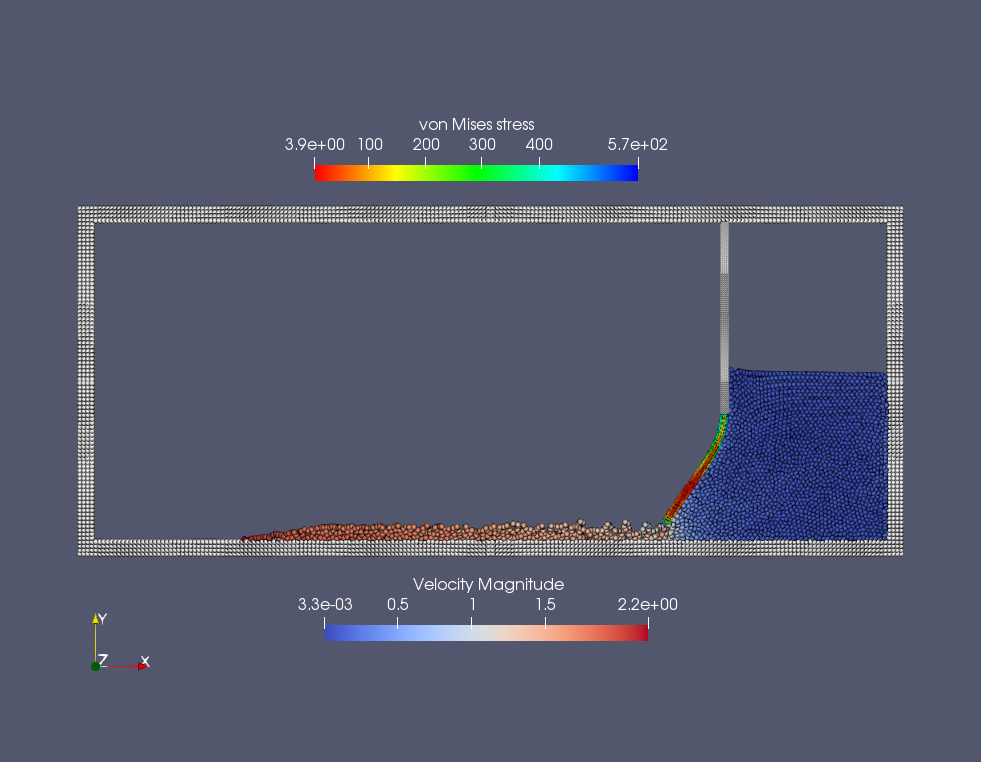
\includegraphics[width=\textwidth]{figs/elastic_gate.png}
	\caption{A snapshot of the particle distribution in the problem of dam break with an elastic gate. }
	\label{figs:elastic-gate}
\end{figure}
%
There are two ways to achieve the constrain. 
One is modeling the base as an elastic body separated from the deformable part 
but constrained the particle motion.
The other way is modeling the entire gate as an elastic body but constrain only the upper base part. 
Here, we choose the first approach.
We give the geometry and material parameters for modeling the elastic gate.
%
\begin{lstlisting}[basicstyle=\ttfamily\footnotesize]
/**
* @brief 	Define the corner point of gate base geomerty.
*/
Vec2d BaseP_lb(DL - Dam_L - Rubber_width, Base_bottom_position); 	/**< Left bottom. */
Vec2d BaseP_lt(DL - Dam_L - Rubber_width, DH); 						/**< Left top. */
Vec2d BaseP_rt(DL - Dam_L, DH); 									/**< Right top. */
Vec2d BaseP_rb(DL - Dam_L, Base_bottom_position); 					/**< Right bottom. */
/**
* @brief 	Define the corner point of gate geomerty.
*/
Vec2d GateP_lb(DL - Dam_L - Rubber_width, 0.0); 					/**< Left bottom. */
Vec2d GateP_lt(DL - Dam_L - Rubber_width, Base_bottom_position); 	/**< Left top. */
Vec2d GateP_rt(DL - Dam_L, Base_bottom_position); 					/**< Right top. */
Vec2d GateP_rb(DL - Dam_L, 0.0); 									/**< Right bottom. */
/**
* @brief Material properties of the elastic gate.
*/
Real rho0_s = 1.1; 						/**< Reference density of gate. */
Real poisson = 0.47; 					/**< Poisson ratio. */
Real Ae = 7.8e3; 						/**< Normalized Youngs Modulus. */
Real Youngs_modulus = Ae * rho0_f * U_f * U_f;
\end{lstlisting}
% 
and define gate bodies and their initial with following code piece.
%
\begin{lstlisting}[basicstyle=\ttfamily\footnotesize]
/**
* @brief  Gate base body definition.
*/
class GateBase : public ElasticBody
{
public:
	GateBase(SPHSystem &system, string body_name, ElasticSolid* material,
		ElasticBodyParticles &elastic_particles,
		int refinement_level, ParticlesGeneratorOps op)
		: ElasticBody(system, body_name, material, elastic_particles,
			refinement_level, op)
	{
		/** Geometry definition. */
		std::vector<Point> gate_base_shape;
		gate_base_shape.push_back(BaseP_lb);
		gate_base_shape.push_back(BaseP_lt);
		gate_base_shape.push_back(BaseP_rt);
		gate_base_shape.push_back(BaseP_rb);
		gate_base_shape.push_back(BaseP_lb);
		body_region_.add_geometry(new Geometry(gate_base_shape), RegionBooleanOps::add);
		/** Finish the region modeling. */
		body_region_.done_modeling();
	}
	/**
	* @brief 	Initialize every gate base particle data.
	*/
	void InitialCondition()
	{
		SetAllParticleAtRest();
	}
};
/**
* @brief  Define the elastic gate body.
*/
class Gate : public ElasticBody
{
public:
	Gate(SPHSystem &system, string body_name, ElasticSolid* material,
		ElasticBodyParticles &elastic_particles,
		int refinement_level, ParticlesGeneratorOps op)
		: ElasticBody(system, body_name, material, elastic_particles,
			refinement_level, op)
	{
		/** Geomerty definition. */
		std::vector<Point> gate_shape;
		gate_shape.push_back(GateP_lb);
		gate_shape.push_back(GateP_lt);
		gate_shape.push_back(GateP_rt);
		gate_shape.push_back(GateP_rb);
		gate_shape.push_back(GateP_lb);
		body_region_.add_geometry(new Geometry(gate_shape), RegionBooleanOps::add);
		/** Finish the region modeling. */
		body_region_.done_modeling();
	}
	/**
	* @brief 	Initialize every elastic gate particle data.
	*/
	void InitialCondition()
	{
		SetAllParticleAtRest();
	}
};
\end{lstlisting}
%
Initially, all particles have been set to at rest.

In the main function, we create the \texttt{SPHBody}s of \texttt{gate\_base} and \texttt{gate} by following piece of code.  
%
\begin{lstlisting}[basicstyle=\ttfamily\footnotesize]
	/**
* @brief 	Material property, particle and body creation of gate base.
*/
ElasticSolid 			solid_material("ElasticSolid", rho0_s, Youngs_modulus, poisson);
ElasticBodyParticles 	gate_base_particles("GateBase");
GateBase *gate_base = new GateBase(system, "GateBase", &solid_material,
gate_base_particles, 1, ParticlesGeneratorOps::lattice);
/**
* @brief 	Material property, particle and body creation of elastic gate.
*/
ElasticBodyParticles 	gate_particles("Gate");
Gate *gate = new Gate(system, "Gate", &solid_material,
gate_particles, 1, ParticlesGeneratorOps::lattice);
\end{lstlisting}
%
Note that the parts of the gate share the same material properties.

Then, the topological relation of all bodies is defined by
%
\begin{lstlisting}[basicstyle=\ttfamily\footnotesize]
	/**
* @brief 	Body contact map.
* @details The contact map gives the data conntections between the bodies.
* 			Basically the the rang of bidies to build neighbor particle lists.
*/
SPHBodyTopology body_topology = { { water_block, { wall_boundary, gate_base, gate } },
	{ wall_boundary, { } },{ gate_base, { gate } },
	{ gate, { gate_base, water_block} }, { gate_observer,{ gate } } };
\end{lstlisting}
%
Here, the \texttt{water\_block} interacts with \texttt{wall\_boundary}, \texttt{gate\_base} and \texttt{gate}, 
the \texttt{gate\_base} with \texttt{gate}, the \texttt{gate} with \texttt{gate\_base} and \texttt{water\_block} and the \texttt{gate\_observer} only with \texttt{gate}. 

After create the bodies, the method related with solid dynamics and FSI will be defined.
First, the method will be used only once.
%
\begin{lstlisting}[basicstyle=\ttfamily\footnotesize]
	/** Initialize normal direction of the wall boundary. */
solid_dynamics::NormalDirectionSummation 	get_wall_normal(wall_boundary, {});
/** Initialize normal direction of the gate base. */
solid_dynamics::NormalDirectionSummation 	get_gate_base_normal(gate_base, { gate });
/** Initialize normal direction of the elastic gate. */
solid_dynamics::NormalDirectionSummation 	get_gate_normal(gate, { gate_base });
/** Corrected strong configuration. */
solid_dynamics::CorrectConfiguration 		gate_base_corrected_configuration_in_strong_form(gate_base, { gate });
solid_dynamics::CorrectConfiguration 		gate_corrected_configuration_in_strong_form(gate, { gate_base });
\end{lstlisting}
%
These are the methods for computing thr normal direction, 
and the reproducing kernel for correcting the SPH approximation of the deformation tensor,
as discussed in Chapter \ref{theory}.

Then the methods which will be used multiple times for solid dynamics are defined.
%
\begin{lstlisting}[basicstyle=\ttfamily\footnotesize]
/**
* @brief Algorithms of Elastic dynamics.
*/
/** Compute time step size of elastic solid. */
solid_dynamics::ElasticSolidTimeStepSize 	gate_computing_time_step_size(gate);
/** Stress relaxation stepping for the elastic gate. */
solid_dynamics::StressRelaxation 			gate_stress_relaxation(gate, { gate_base });
/** Stress update for contrained wall body(gate base). */
solid_dynamics::StressInConstrinedElasticBodyFirstHalf 	gate_base_stress_update_first_half(gate_base, { gate });
solid_dynamics::StressInConstrinedElasticBodySecondHalf gate_base_stress_update_second_half(gate_base, { gate });
/** Update the norm of elastic gate. */
solid_dynamics::UpdateElasticNormalDirection 	gate_update_normal(gate);
/** Compute the average velocity of gate. */
solid_dynamics::InitializeDisplacement 			gate_initialize_displacement(gate);
solid_dynamics::UpdateAverageVelocity 			gate_average_velocity(gate);
\end{lstlisting}
%
We still need define the method for FSI, which computes the pressure force acting on solid particles.
%
\begin{lstlisting}[basicstyle=\ttfamily\footnotesize]
/**
* @brief Algorithms of FSI.
*/
/** Compute the force exerted on elastic gate due to fluid pressure. */
solid_dynamics::FluidPressureForceOnSolid 	fluid_pressure_force_on_gate(gate, { water_block }, &fluid, &gravity);
\end{lstlisting}
%
The main loops are defined in the following piece of code.
%
\begin{lstlisting}[basicstyle=\ttfamily\footnotesize]
/**
* @brief Main loop starts here.
*/
while (GlobalStaticVariables::physical_time_ < End_Time)
{
	Real integeral_time = 0.0;
	/** Integrate time (loop) until the next output time. */
	while (integeral_time < D_Time)
	{
		Dt = get_fluid_adevction_time_step_size.parallel_exec();
		update_fluid_desnity.parallel_exec();
		/** Acceleration due to viscous force and gravity. */
		initialize_fluid_acceleration.parallel_exec();
		add_fluid_gravity.parallel_exec();
		/** Update normal direction on elastic body. */
		gate_update_normal.parallel_exec();
		Real relaxation_time = 0.0;
		while (relaxation_time < Dt)
		{
			if (ite % 100 == 0) {
				cout << "N=" << ite << " Time: "
				<< GlobalStaticVariables::physical_time_ << "	dt: "
				<< dt << "\n";
			}
			/** Fluid relaxation and force computaton. */
			pressure_relaxation.parallel_exec(dt);
			fluid_pressure_force_on_gate.parallel_exec();
			/** Solid dynamics time stepping. */
			Real dt_s_sum = 0.0;
			gate_initialize_displacement.parallel_exec();
			while (dt_s_sum < dt)
			{
				Real dt_s = gate_computing_time_step_size.parallel_exec();
				if (dt - dt_s_sum < dt_s) dt_s = dt - dt_s_sum;
				if (ite % 100 == 0) {
					cout << "N=" << ite << " Time: "
					<< GlobalStaticVariables::physical_time_ << "	dt_s: "
					<< dt_s << "\n";
				}
				gate_base_stress_update_first_half.parallel_exec(dt_s);
				gate_stress_relaxation.parallel_exec(dt_s);
				gate_base_stress_update_second_half.parallel_exec(dt_s);
				dt_s_sum += dt_s;
			}
			gate_average_velocity.parallel_exec(dt);
			
			ite++;
			dt = get_fluid_time_step_size.parallel_exec();
			relaxation_time += dt;
			integeral_time += dt;
			GlobalStaticVariables::physical_time_ += dt;
		}
		/** Update cell linked list and configuration. */
		update_water_block_cell_linked_list.parallel_exec();
		update_water_block_configuration.parallel_exec();
		update_gate_cell_linked_list.parallel_exec();
		update_gate_interaction_configuration.parallel_exec();
		/** Output the observed data. */
		write_beam_tip_displacement.WriteToFile(GlobalStaticVariables::physical_time_);
	}
	tick_count t2 = tick_count::now();
	write_real_body_states_to_vtu.WriteToFile(GlobalStaticVariables::physical_time_  * 0.001);
	tick_count t3 = tick_count::now();
	interval += t3 - t2;
}
\end{lstlisting}
%
Note that, since data exchanging frequency for FSI is defined 
by the acoustic time step of fluid computation, 
we need computed the time averaged velocity of elastic particles during this period.
Beside the particle position, pressure and stress distribution, 
we output the displacement of the gate tip,
as shown in Fig. \ref{figs:elastic-gate-tip}.
%
\begin{figure}[tb!]
	\centering
	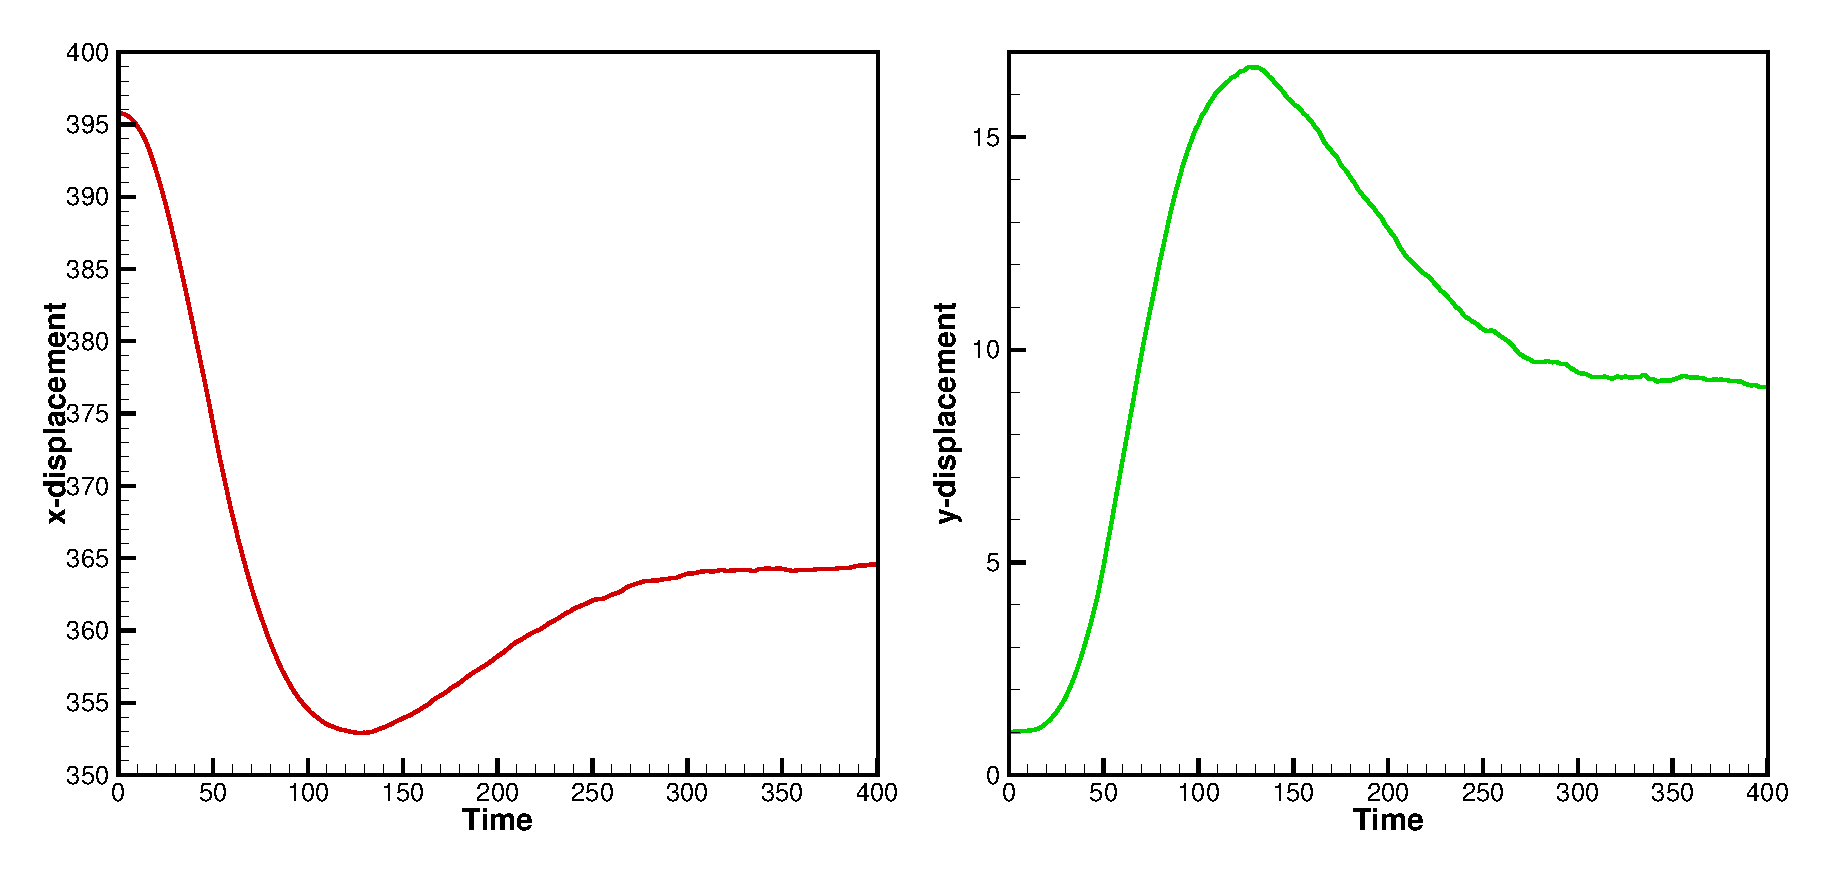
\includegraphics[width=\textwidth]{figs/displacement.eps}
	\caption{Temporal displacement of the tip point on the elastic gate.}
	\label{figs:elastic-gate-tip}
\end{figure}
%
We should mention that we can add new features 
to the methods related with the observer for more quantitative information the simulation.

\bibliographystyle{plain}
\bibliography{sphinxsys}
\end{document}

